\documentclass[a4paper, 11pt]{report}

%============================ PACKAGES ============================
%%%%%%%%%%%%%%%%%%%%%%%%%%%%%%%%%%%%%%%%
%           Liste des packages         %
%%%%%%%%%%%%%%%%%%%%%%%%%%%%%%%%%%%%%%%%

\usepackage[frenchb]{babel}
\usepackage[utf8]{inputenc}
\usepackage{lmodern}
\usepackage[T1]{fontenc}
\usepackage[top=2.5cm, bottom=2.5cm, left=2.5cm, right=2cm]{geometry}
\usepackage{graphicx}
\usepackage{float}
\usepackage{setspace}
\usepackage{amsmath}
\usepackage{xcolor}
\usepackage{hyperref}
\usepackage[french,onelanguage]{algorithm2e}
\usepackage{ae,aecompl}		% Utilisation des fontes vectorielles modernes
\usepackage{eso-pic}        % Facilite le positionnement des images de manière absolu
\usepackage{booktabs}
\usepackage[]{siunitx}
\usepackage[upright]{fourier}
\usepackage{fancyhdr}
\usepackage[automake]{glossaries-extra}
\usepackage[nottoc]{tocbibind}
\usepackage{etoolbox}
%======================== COMMANDES ========================
\patchcmd{\chapter}{\thispagestyle{plain}}{\thispagestyle{fancy}}{}{}
\setlength{\headheight}{26pt}
\pagestyle{fancy}
\renewcommand{\headrulewidth}{1pt}
\fancyhead[L]{\leftmark}
\fancyhead[R]{}
\renewcommand{\footrulewidth}{1pt}
\fancyfoot[C]{\textbf{\thepage}} 
\fancyfoot[L]{}
\fancyfoot[R]{} 
\newcommand{\HRule}{\rule{\linewidth}{0.5mm}}
\graphicspath{{./ressources/}}
\makeglossaries

%======================== INFOS DE LA PAGE DE GARDES ========================
% Infos de la page de garde

%%%%%%%%%%%%%%%%%%%%%%%%%%%%%%%%%%%%%%%%%%
%           Page de Garde		         %
%%%%%%%%%%%%%%%%%%%%%%%%%%%%%%%%%%%%%%%%%%

\makeatletter
\def\@ecole{école}
\newcommand{\ecole}[1]{
	\def\@ecole{#1}
}

\def\@specialite{Spécialité}
\newcommand{\specialite}[1]{
	\def\@specialite{#1}
}

\def\@faculte{Faculté}
\newcommand{\faculte}[1]{
	\def\@faculte{#1}
}

\def\@filiere{Filière}
\newcommand{\filiere}[1] {
	\def\@filiere{#1}
}

\def\@dept{Département}
\newcommand{\dept}[1]{
	\def\@dept{#1}
}

\def\@domaine{Domaine}
\newcommand{\domaine}[1]{
	\def\@domaine{#1}
}

\def\@directeur{directeur}
\newcommand{\directeur}[1]{
	\def\@directeur{#1}
}

\def\@helper{helper}
\newcommand{\helper}[1]{
	\def\@helper{#1}
}

\def\@jurya{}{}{}
\newcommand{\jurya}[3]{
	\def\@jurya{#1,	& #2	& #3\\}
}
\def\@juryb{}{}{}
\newcommand{\juryb}[3]{
	\def\@juryb{#1,	& #2	& #3\\}
}
\makeatother

\makeatletter
\newcommand{\pagedegarde}{
	\thispagestyle{empty}
	\begin{titlepage}
		\begin{tikzpicture}[remember picture,overlay]
			\draw[very thick]
			([yshift=-1cm,xshift=2cm]current page.north west)--
			([yshift=-1cm,xshift=-1cm]current page.north east)--
			([yshift=1cm,xshift=-1cm]current page.south east)--
			([yshift=1cm,xshift=2cm]current page.south west)--cycle;
		\end{tikzpicture}
		\hspace{4}
		
\includegraphics[width=0.15\textwidth]{USTHBLogo.png}
		\hspace{12}
		\large {\bfseries{ République Algérienne Démocratique et Populaire }}
		\hspace{8}
		
\includegraphics[width=0.15\textwidth]{USTHBLogo.png}
		
		
		\centering{
			{\bfseries Ministère de l'Enseignement Supérieur et de la Recherche Scientifique}\\}
		\vspace{0.5cm}
		{\Large
			{\bfseries \@ecole}\\
			\vspace{0.25cm}
			
			\vspace{0,5cm}
			{\bfseries Faculté \@faculte}\\
			{\bfseries Département \@dept}\\
		}\\
		
		\vspace{0.5cm}
		
		\large M\'{E}MOIRE DE LICENCE\\
		
		\vspace{0.75cm}

		{\large \textit{Domaine} : \bfseries {\@domaine}}\\
		{\large \textit{Filière} : \bfseries {\@filiere}}\\
		{\large \textit{Spécialité} : \bfseries{\@specialite}}\\
		\vspace{0.5cm}
		\HRule \\[0.4cm]
		{\huge{\bfseries{Thème}}}\\
		\vspace{0.25cm}
		{\Huge \color[RGB]{18,96,149} \bfseries{\@title}\\[0.4cm] }
		\HRule \\[0.3cm]
		\vfill
		\vspace{0.3cm}
		\textit{Réalisé par}\\
		\vspace{0.125cm}
		{\Large {\bfseries \@author}} \\
		\vspace{0.125cm}
		\textit{et}\\
		\vspace{0.125cm}
		{\Large {\bfseries \@helper}} \\
		\vspace{0.5cm}
		\textit{Soutenu le} : {\bfseries \@date} \\
		\vfill
		\vspace{0.25cm}
		
		\large \textit{Devant le jury composé de\\}
		\vspace{0.25cm}
		\begin{tabular}{>{\bfseries}llr}
			
			\@jurya
			\@juryb
			%\@juryc
		\end{tabular}
		\vfill
		\vspace{0.5cm}
		Dirigé par : {\bfseries \@directeur}\\
		\vfill
		\vspace{0.25cm}
		\textbf{Binôme \No 047/21}
		
	\end{titlepage}
	\restoregeometry  
}
\makeatother

\author{Ayoub \scshape{HAMMAL}}
\helper{ Mehdi \scshape{LERARI}}
\title{Conception et implémentation d'une
technique d'allocation de ressources dans un environnement \emph{Fog Computing}}
\specialite{Réseaux et Systèmes Distribués}
\domaine{Mathématiques et Informatique}
\filiere{Informatique}
\dept{d'Informatique}
\faculte{d'\'{E}lectronique et d'Informatique} 
\directeur{Dr. Khaled \scshape{ZERAOULIA}}
\date{XX XXX 2021}
\jurya{XXXX \scshape{YYYY}}{ }{Président du jury}
\juryb{XXXX \scshape{YYYY}}{ }{Membre du jury}
\ecole{Université des Sciences et de la Technologie \scshape{Houari Boumédiène}}
%======================== Méta-données du PDF ======================
\hypersetup{
    	pdfauthor={Ayoub HAMMAL et Mehdi LERARI},
    	pdfsubject={Mémoire de Licence},
    	pdftitle={Conception et implémentation d'une
	technique d'allocation de ressources dans un environnement Fog Computing},
    	pdfkeywords={XXXX,XXXX,XXXX,XXXX,XXXX},
	}
%======================== Glossaire ================================
\newacronym{IoT}{IoT}{signifie Internet of Things (ou Internet des objets)}
\newglossaryentry{latence}{
	name={Latence},
	description={Temps nécessaire à un paquet de données pour passer de la source à la destination à travers un réseau},
}
\newglossaryentry{Fog Computing}{
	name={Fog Computing},
	description={Technologie Cloud dans laquelle les données générées par les terminaux ne sont pas directement téléchargées dans le cloud, mais sont au préalable prétraitées dans des mini-centres de calcul décentralisés},
}
\newglossaryentry{Cloud Computing}{
	name={Cloud Computing},
	description={Correspond à l’accès à des services informatiques via Internet à partir d’un fournisseur de services},
}
\newglossaryentry{virtualisation}{
	name={Virtualisation},
	description={Technologie qui permet de créer plusieurs environnements simulés ou ressources dédiées à partir d'un seul système physique},
}
\newglossaryentry{machine virtuelle}{
	name={Machine Virtuelle},
	description={Environnement virtuel qui fonctionne comme un système informatique virtuel, avec son propre processeur, sa mémoire, son interface réseau et son espace de stockage, mais qui est créé sur un système matériel physique},
}
\newglossaryentry{conteneur}{
	name={Conteneur},
	description={Enveloppe virtuelle qui permet de distribuer une application avec tous les éléments dont elle a besoin pour fonctionner : fichiers source, environnement d'exécution, librairies, outils et fichiers},
}
\newglossaryentry{migration}{
	name={Migration},
	description={Processus qui consiste à déplacer l'état d'une instance virtuelle, d'un hôte physique à un autre}
}
%======================== Début du document ========================
\begin{document}

%Page de garde
\pagedegarde
%table des matières
\tableofcontents
%liste des figures
\listoffigures
\thispagestyle{fancy}
%liste des abréviations et glossaire
\printglossary
\thispagestyle{fancy}

\chapter{Introduction générale}
L'Internet des objets est un sujet émergent d'importance technique, sociale et économique. Les produits de consommation, les biens durables, les voitures, les composants industriels et utilitaires, les capteurs et autres objets du quotidien sont combinés à la connectivité Internet et à de puissantes capacités d'analyse de données qui promettent de faciliter tous les aspects de notre vie. La perspective d’une vie quotidienne plus confortable, d’une économie et d’une administration plus efficaces, d'une circulation routière plus sûre, d’un approvisionnement énergétique plus respectueux de l'environnement et d’une vie plus saine favorise son développement. Une production industrielle plus pe, des voitures autonomes et des bracelets qui détectent et signalent immédiatement les maladies, les applications possibles couvrent un large éventail de domaines de la vie. De nombreuses activités peuvent être mieux planifiées sur la base des données collectées par les machines en réseau. Les projections de l'impact de l'\emph{IoT} sur Internet et l'économie sont impressionnantes, certains prévoyant jusqu'à 100 milliards d'objets connectés IoT et un impact économique mondial de plus de 11 milliards de dollars d'ici 2025. \par
La croissance fulgurante du nombre d'objets connectés ainsi que la quantité de donnés généré et par ces derniers ont mis évidence certains problèmes liés au Cloud Computing, et particulièrement à son architecture centralisée. Nous pouvons citer par exemple le problème de surcharge, ou encore la dégradation des performances réseau.\\
Pour pallier à ces problèmes, une alternative au paradigme Cloud a été proposée en 2012 se présentant comme étant une extension de ce dernier nommé "Fog Computing". Cette nouvelle approche permet de décharger le Cloud d'une partie des services qu'il propose en utilisant les capacités limitées dont disposent les ressources intermédiaires entre les objets connectés et le Cloud, d'où le terme Fog.\\ 
Pour cette raison, le Fog Computing semble être un moyen prometteur pour améliorer les performances réseau, limiter les points de surcharges et réduire la latence, ce qui permet de répondre aux exigences de certaines applications sensibles à l'état du réseau, notamment les applications à temps réel.\\
Cependant, le passage du Cloud Computing au Fog Computing n’est pas si simple. Les ressources
intermédiaires ayant des capacités limitées, il est important de disposer d'un mécanisme de gestion de ressource permettant de gérer efficacement les ressources disponibles.
\par
Dans ce travail, nous proposons une nouvelle technique d'allocation de ressources dans un environnement \emph{Fog/Edge Computing} visant à servir de manière optimale les demandes de services générées par un ensemble d'objets \emph{IoT}. Nous exploitons dans cette technique l'algorithme de correspondance de Gale-Shapley prouvé stable et efficace.\\
Nous commencerons d'abord par définir les concepts clés de la problématique et établir l'état de l'art concernant ce domaine de recherche. Puis dans un second chapitre, nous présenterons notre technique, le scénario d'exécution et les différents échanges entre les entités de notre environnement. Enfin, nous proposerons dans le dernier chapitre une implémentation de cette technique dans un environnement de simulation, ainsi qu'une discussion et une analyse des résultats obtenus.
\chapter{Généralités}

\section{Introduction}
Nous présentons dans ce chapitre les principaux concepts liés au \emph{\gls{Fog Computing}}. Nous commençons d'abord par introduire l'Internet des objets et leur relation au Fog Computing. Puis, nous expliquons les techniques de migration de conteneurs entre les nœuds Fog. Enfin, nous terminons ce chapitre par une taxonomie des travaux similaires axés sur la gestion de ressources des nœuds Fog, ainsi que les différents défis rencontrés. 

\section{Internet des objets (IoT)}
\subsection{Définition}
Le terme Internet des objets (Internet of Things ou \emph{\gls{IoT}}) décrit le réseau d'appareils physiques - souvent hétérogène - interconnectés, et dont le rôle principal est la récolte et l'échange d'information, ainsi que l'interaction avec l'environnement extérieur \cite{patel2016}. Cette infrastructure est dite intelligente, dotée de la capacité de s'auto-organiser, partager l'information de manière optimale et de réagir aux changements environnementaux \cite{madakam2015}.\par
Les objets dans ce type de réseau sont de capacité limitée, que ce soit en puissance de calcul ou en consommation d'énergie. Ce sont majoritairement des objets électroniques quotidiens (à l'exemple de smartphones, véhicules ou équipements ménagers), chacun avec sa propre identité pour communiquer avec le reste des objets et synchroniser les efforts de réponses aux différentes situations externes auxquelles ils sont exposés.

\subsection{Histoire et Évolution}
L'idée d'interconnecter des dispositifs électroniques moyennant un réseau informatique est apparue dans les années 80s, à l'Université de Carnegie Melon, où on avait relié un distributeur de boissons fraîches à un ordinateur de monitorage. Ce qui a permis aux programmeurs de consulter la disponibilité des boissons à distance et d'éviter les trajets inutiles \cite{madakam2015}.\par
Cependant, le premier à avoir introduit ce concept est Kevin Ashton en 1999, qui travaillait dans l'optimisation de chaîne de production chez Procter \& Gamble. Ashton avait constaté qu'en 1999, 50 petabytes d'information étaient créés par des êtres humains. D'où, il a dévelopé l'idée de décharger l'homme de cette tâche fastidieuse de récolte d'information et ce, lors d'une présentation portant le nom de la technologie (Internet of Things). Il propose plutôt d'exploiter la masse d'engins et de capteurs disponibles et déjà déployés à ce moment là \cite{ashton2009}.\par
Cette infrastructure n'a été adoptée en industrie qu'en fin de l'année 2000s. Depuis, les constructeurs du domaine de téléinformatique concentrent leurs efforts sur la production de capteurs et d'appareils IoT avec différentes fonctionnalités dans le but de combler les besoins des diverses industries, allant de l'agriculture et domaine médical jusqu'à l'industrie militaire.

\subsection{Architecture}
L'architecture d'un réseau IoT se décompose en 4 couches flexibles. Chaque couche est constituée de plusieurs technologies et standards \cite{patel2016}. Cet aspect modulaire permet une meilleure scalabilité de l'infrastructure et une meilleure adaptation aux besoins émergeants. Les couches de ce modèle sont comme suit:
\begin{enumerate}
  \item \emph{La couche de capteurs et d'objets intelligents:} Elle est formée d'objets connectés munis de capteurs et/ou d'actionneurs. C'est la couche la plus proche de l'environnement physique, celle-ci transforme les événements générés par ce dernier en un flux d'information à temps réel, et se charge de leur transmission. Les capteurs ont différentes spécifications, comme la mesure de la température, ou la pression, la capture de mouvement …, et sont connectés soit à des passerelles à l'aide de réseaux filaires (Ethernet) ou non (Wi-Fi, Bluetooth, RFID …), soit directement à la couche applicative. Un exemple de ce type de technologie est les WSNs, caractérisés par leur basse consommation d'énergie et grande zone de couverture.
  \item \emph{La couche réseau et passerelles:} Cette couche garantit la transmission de la masse d'information générée par la couche précédente, tout en respectant la qualité de service exigée par les applications servies. Plusieurs infrastructures et protocoles de communication ont été mis en place dans le but d'optimiser l'acheminement et traitement d'information, comme le concept de Fog Computing qu'on détaillera par la suite.
  \item \emph{La couche de gestion:} Le rôle de cette couche est de filtrer et organiser les informations, en fournissant une couche d'abstraction à l'application. Elle s'occupe de la gestion de priorité, et l'analyse de la pertinence des données. C'est aussi à ce niveau que les politiques d'anonymisation et sécurisation de données sont implémentées.
  \item \emph{La couche d'application:} Elle est située majoritairement dans des clouds ou data-centers. Les applications couvrent des domaines différents comme l'agriculture et la gestion de villes intelligentes, et d'autres plus critiques, comme le domaine de la santé ou le domaine militaire. Toutefois, depuis quelques années, les efforts de recherche visent à rapprocher ces applications de la première couche du modèle, pour des motifs que nous expliquerons dans la section dédiée au Fog Computing. 
\end{enumerate}

\subsection{Quelques domaines d'application}
L'installation d'objets intelligents s'est démocratisée depuis quelques années. On les retrouve dans les environnements suivants:
\begin{itemize}
  \item Les systèmes de sécurité et surveillance, où des caméras et capteurs de mouvements permettent de détecter et identifier toute activité suspecte.
  \item Les maisons intelligentes: ce qui décrit la connectivité des objets dans un domicile, tous œuvrent pour fournir de meilleures conditions de vie, et ceci en assurant: la régulation de températures, l'optimisation de consommation d'énergie, la détection d'incendie et le filtrage de l'air.
  \item Les systèmes de voitures autonomes dans lesquels les véhicules utilisant la voie publique peuvent s'échanger des informations, parfois critiques, et alerter les conducteurs de tout danger imminent. Ils peuvent aussi, en se basant sur les informations de géolocalisation fournies par les autres usagers, produire des recommandations de destination tout en évitant les points de congestion de la circulation routière.
  \item Les dispositifs permettant la surveillance médicale de personnes incapacités, et ainsi la prise de dispositions nécessaires dans les moments d'urgence.
\end{itemize}

\subsection{Problèmes et difficultés}
Le provisionnement en énergie est devenu une des préoccupations de la société actuelle. On cherche à optimiser l'utilisation de ressources énergétiques, soit pour étendre l'autonomie des objets et capteurs mobiles, ou bien pour réduire les frais d'approvisionnement en électricité. Des algorithmes de gestion et allocation des ressources ont été proposés pour minimiser cette consommation, mais les recherches sur ce sujet sont toujours actives.\par
Avec la croissance du nombre d'objets connectés, les attaques cybercriminelles deviennent excentriques. Ce réseau peut être vulnérable contre l'injection de données erronées qui peuvent influencer des prises de décision parfois critiques. Les nœuds intercommunicants disposent de ressources limitées, et ainsi, ils peuvent être sujets à des attaques de déni de service (\emph{DDOS}). La grande quantité de données produite doit être protégée tout au long du circuit liant les couches présentées précédemment. Un travail de supervision doit être mené dans le but de garantir la confidentialité des données récoltées, et empêcher les pratiques abusives comme la vente de données d'utilisateurs \cite{COLAKOVIC201817}.\par
De plus, certaines applications demandent une certaine réactivité et une grande vitesse de réponse pour accomplir des missions critiques comme pour la conduite de véhicules automobiles ou la surveillance médicale. Ces exigences sont souvent restreintes par d'autres contraintes comme la mobilité des objets connectés ou la congestion dans le réseau de communication.
%------------------------------------------------------------
\section{Fog Computing}

\subsection{Histoire et évolution}
Malgré les avantages considérables que procure le \emph{\gls{Cloud Computing}} en termes de performance, d'accessibilité et de scalabilité, Ce dernier se heurte néanmoins à quelques limites face à l'expansion de l'Internet des objets (IoT), ce qui impose donc une réévaluation de ce paradigme. \par 
En effet, l'accélération de la croissance du nombre d'appareils connectés à Internet ainsi que l'énorme quantité de données générées par ces derniers ont démontré une certaine limitation du paradigme Cloud. Le problème le plus apparent est le problème de \emph{\gls{latence}}, en vue donc de la croissance de la quantité de données générées par les différents objets connectés et la dépendance de ces derniers visés à vis du Cloud pour le traitement de ces données, ceci risque de provoquer une réduction considérable des performances du réseau, ce qui engendrerait une augmentation des délais de transfert et donc une diminution des performances de traitement. Ce qui peut être critique au niveau de certaines applications notamment les applications qui requièrent des traitements en temps réel.\\
D'autres problèmes peuvent être cités également, comme le problème de congestion ou encore le problème de connaissance de localisation. \par
C'est pour répondre donc à ces problèmes que le Fog Computing a été proposée comme une extension du paradigme Cloud en 2012, et qui a vu par la suite la création d'un consortium dédié qu'est l'\textbf{OpenFog Consortium} afin de faciliter l'interopérabilité des différentes solutions technologiques.

\subsection{Définition et concept}
Selon la définition proposée par CISCO \cite{bonomi2012}, le terme Fog computing désigne : \og{}une plate-forme hautement virtualisée qui fournit des services de calcul, de stockage et de mise en réseau entre les appareils finaux et les centres de données de Cloud Computing traditionnels, généralement, mais pas exclusivement, située à la périphérie du réseau\fg{}.\par
L'\emph{OpenFog Consortium} \cite{OpenFog2017} le définit aussi comme étant : \og{} Une architecture horizontale au niveau du système qui distribue des fonctions de calcul, de stockage, de contrôle et de mise en réseau plus proches des utilisateurs le long du continuum Cloud-objet\fg{}.\par
Le terme réfère aussi à une infrastructure matérielle et applicative distribuée qui vise à stocker et à traiter les données issues des différents appareils connectés afin de se substituer au Cloud pour certains traitements.\par
La principale idée du Fog Computing est l'instrumentalisation des différents équipements qui constitue les noeuds du réseau (routeurs, commutateurs, passerelles, etc.) comme étant un centre de traitement et de stockage de donnés distribué qui est à la fois intermédiaire au Cloud et en même temps proche des extrémités du réseau.
En créant donc une couche auprès de la production des données, ceci entraîne une réduction des transferts entrant et sortant du Cloud et donc une réduction de la latence, et par conséquent du temps des différents traitements et services.

\subsection{Architecture}
La plupart des recherches qui s'orientent vers la définition d'un modèle architectural semblent se diriger vers un même modèle, à savoir un modèle en 3 couches \cite{de2019}.\\
Les couches de ce modèle sont présentées comme suit :
\begin{description}
  \item[Couche IoT :] cette couche désigne l'ensemble des appareils se trouvant à l'extrémité du réseau, elle est composée essentiellement d'appareils IoT tels que des véhicules intelligents, des smartphones, des drones militaires, des capteurs sensoriels, etc. Le rôle de ces derniers étant la collecte et la transmission des données vers la couche supérieure pour stockage ou traitement.
  \item[Couche de Fog :] cette couche constitue le point central du paradigme Fog, elle est constituée d'un ensemble de nœuds Fog, qui selon le OpenFog Consortium, ce dernier se définit comme 
  \og{}un élément physique ou logique qui implémente les services informatiques Fog\fg\cite{de2019}.\par
  L'ensemble des nœuds constitue un centre de traitement et de stockage distribué connecté à la fois à la couche inférieure et celle supérieure à travers des nœuds passerelles, permettant ainsi de bénéficier des différents services fournis par la couche supérieure qu'est le Cloud par exemple le stockage, tout en fournissant des informations contextuelles aux utilisateurs au niveau de la couche inférieure.
  \item[Couche cloud :] cette couche représente une infrastructure Cloud centralisée. Elle est composée de ressources matérielles élevées et fournit différents services, ayant comme différences avec une architecture en Cloud classique, certains traitements et services qui sont déchargés de la couche Cloud au profit de la couche Fog afin d'équilibrer la charge de travail et d'augmenter l'efficacité et la fiabilité.
\end{description}

\subsection{Avantages}
Le Fog computing présente de nombreux avantages qu'il convient de souligner, Ils sont généralement résumés sous le sigle SCALE pour :
\begin{itemize}
  \item \emph{Sécurité :} Dans ce paradigme, la sécurité est prise en considération lors de l'élaboration de l'architecture plutôt qu'une partie optionnelle.
  \item \emph{Cognition :} vient du fait que l'infrastructure Fog est consciente des besoins et exigences des utilisateurs. Elle distribue ainsi plus finement les ressources en fonction de chaque utilisateur contrairement au Cloud.
  \item \emph{Agilité :} Ce qui désigne la capacité d'adaptation rapide à l'innovation.
  \item \emph{Latence :} En raison de sa proximité avec les utilisateurs finaux, le Fog a la capacité de supporter des applications qui nécessitent des latences courtes et stables, évitant ainsi les problèmes résultant des systèmes centralisés.
  \item \emph{Efficacité :} vient du fait que cette vision étant les capacités du Cloud en intégrant
  les différents nœuds qui composent le réseau à l'infrastructure de traitement et de stockage, augmentant ainsi la capacité ainsi que l'efficacité globale du système.
\end{itemize}

\subsection{Défis et verrous scientifiques}
Bien que le Fog Computing ait apporté des avantages considérables, ce paradigme reste relativement récent et nécessite  d'investiguer certains défis, par exemple :
\begin{itemize}
  \item \emph{Gestion de l'énergie:} Les infrastructures de Fog comprennent généralement un grand nombre de nœuds géo-distribués. La consommation énergétique est donc plus élevée en comparaison avec celle du Cloud. De grands efforts de recherche sont alors nécessaires pour développer des solutions efficaces afin de minimiser l'empreinte énergétique, par exemple, des algorithmes de traitement et des protocoles de communication moins coûteux en énergie sont à développer.
  \item \emph{Hétérogénéité:} En plus de l'hétérogénéité trouvée dans les environnements IoT, aux nivaux des types d'objets connectés, des données, des technologies de communications et des performances. Ce problème est également présent dans les infrastructures Fog en raison de la diversité des équipements qui constituent les nœuds Fog. La gestion de l'hétérogénéité dans un environnement de Fog et d'IoT représente un défi important.
  \item \emph{Gestion et provision de ressources:} Les noeuds Fog sont généralement des équipements à capacité limités, il est par conséquent indispensable de disposer de solution efficace en termes de gestion de ressource, par exemple l'ordonnancement des différentes applications.
\end{itemize}
%------------------------------------------------------------
\section{Migration dans les environnements Fog Computing}

\subsection{Définitions et concepts}
La \emph{\gls{virtualisation}} introduit une couche d'abstraction logicielle entre le matériel et le système d'exploitation ou les applications qui s'exécutent dessus. En séparant les ressources logiques des ressources physiques sous-adjacentes, la virtualisation permet l'affectation flexible de charges de travail entre les machines physiques.
La \emph{\gls{migration}}d'instance virtuelle (\emph{\gls{machine virtuelle}} ou \emph{\gls{conteneur}}) est considérée comme le processus de copie et déplacement de l'état de cette dernière d'un hôte physique à un autre \cite{boutaba2013}.\par
\subsection{Migration VMs-Conteneurs}
La migration d'instance virtuelle joue un rôle essentiel dans les environnements Fog étant donné qu'elle permet de garantir la continuité des services, quels que soient les besoins en mobilité exprimés par les objets connectés à cet environnement.
Il existe deux grandes techniques de virtualisation logicielle exploitées dans les architectures orientées services: les machines virtuelles et les conteneurs. Leurs principales différences résident dans leur évolutivité et leur portabilité \cite{redhat} (voir Figure \ref{fig:vmvsconteneur}).\par
Dans le cas général, le volume d'un conteneur se compte en mégaoctets. Il ne comporte rien de plus gros qu'une application et ses fichiers qu'elle en dépend. Ce sont des paquets à monofonctionnalité, effectuant des tâches spécifiques (appelées microservices) \cite{redhat}. C'est une méthode de virtualisation au niveau du système d'exploitation(Software Virtualization) qui vise à exécuter plusieurs systèmes totalement isolés (conteneurs) sur un seul hôte de contrôle (un simple système d'exploitation). Les conteneurs partagent le noyau avec l'hôte et fournissent un environnement indépendant qui possède son propre CPU, mémoire, bloc d'E/S, réseau et le mécanisme de contrôle des ressources.\par
D'autre part, une machine virtuelle est plus volumineuse (plusieurs gigaoctets), comporte son propre système d'exploitation y compris son noyau. Elle permet l'exécution simultanée de plusieurs fonctions gourmandes en ressources \cite{microsoft2019}. L'ensemble de machines virtuelles sur une même machine sont gérées par un hyperviseur, qui permet leur isolation en s'exécutant sur des hôtes physiques et il est également responsable de la coexistence de différents noyaux des machines virtuelles au sein d'une même machine physique.\par
Donc la différence principale est que les conteneurs permettent de virtualiser un système d'exploitation afin que plusieurs charges de travail s'exécutent sur un système d'exploitation unique (on peut prendre l'exemple d'une base de données MySQL qu'on aura comme copie individuelle dans une machine virtuelle, mais avec l'utilisation des conteneurs on aura la possibilité d'avoir plusieurs copies des services de ce dernier).\par
Les conteneurs partagent en pratique le même noyau du système d'exploitation hôte contrairement aux technologies de machines virtuelles où le matériel est virtualisé pour exécuter plusieurs instances de système d'exploitation. Cela permet de lancer un nombre beaucoup plus important de conteneurs que de machines virtuelles sur le même matériel, et ainsi fournir une haute disponibilité capable de satisfaire la demande imposée par les réseaux de nouvelle génération telle que la 5G. Des exemples de systèmes à base de conteneurs sont Docker, OpenVZ, LXC et LXD. 
\begin{figure}[H]
\centering
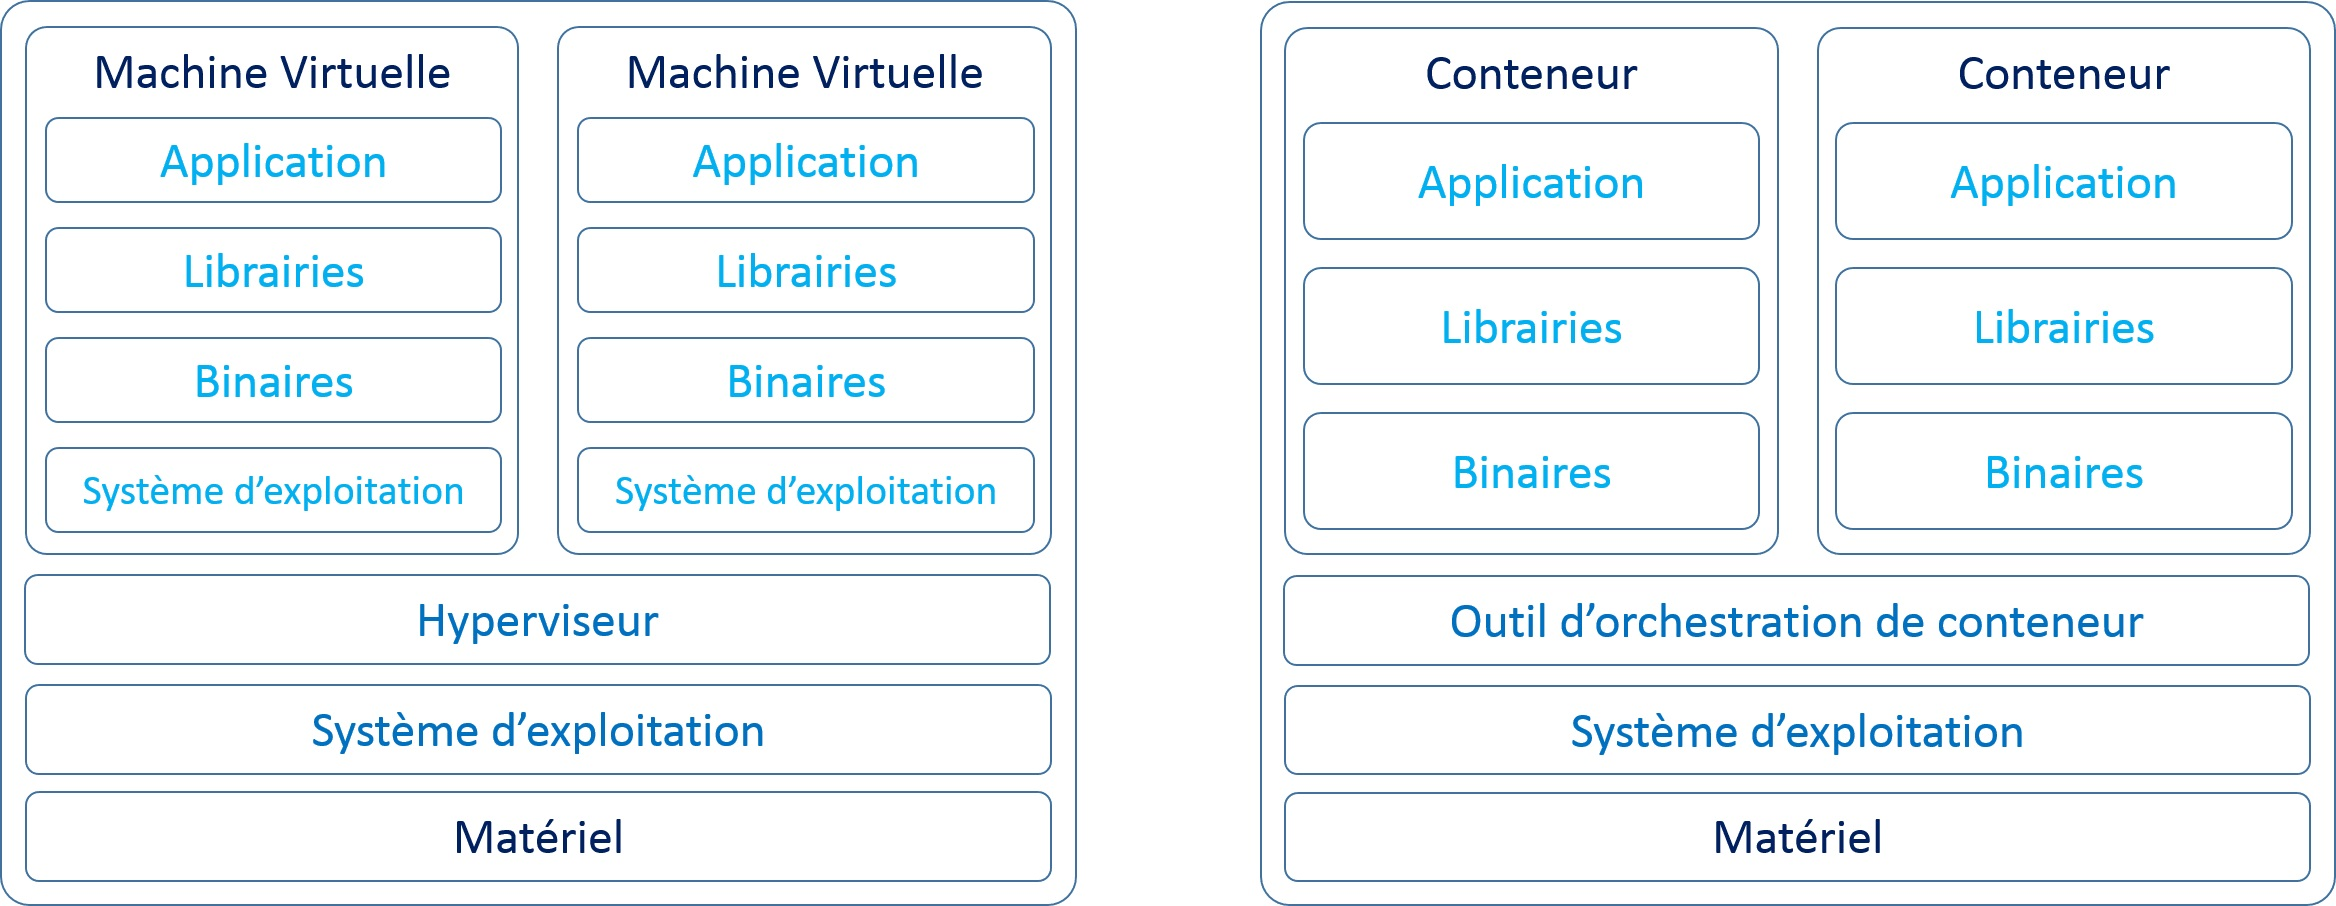
\includegraphics[scale=0.2]{vm-container.jpg}
\caption{Architecture de machine virtuelle, et de conteneur \cite{alibabacloud}}
\label{fig:vmvsconteneur}
\end{figure}

\subsection{Avantages et inconvénients}
\subsubsection{Avantages de la virtualisation et de la migration}
La dynamicité de ce mécanisme de migration confère une flexibilité dans la distribution et organisation des tâches de travail sur l'ensemble des ressources matérielles. Cela permet de répondre efficacement aux fluctuations des charges en mobilisant les conteneurs et machines virtuelles selon le besoin. Deux utilisations sont envisageables comme suit \cite{boutaba2013}.\par
D'une part, la migration permet de consolider les serveurs, en regroupant les instances virtuelles sur un nombre réduit de machines. Cette utilisation est particulièrement efficace dans le scénario de charge réduite et considérablement inférieure à la capacité de traitement totale disponible. Ceci afin de permettre la mise en veille ou la suspension des machines non exploitées et en l'occurrence réduire la consommation énergétique et ainsi les coûts engendrés.\par
D'une autre part, et dans les conditions opposées à celles susmentionnées, c'est-à-dire dans un environnement qui exige de grandes capacités de traitement, la précédente technique cause une surcharge sur les machines exploitées et par la suite une dégradation du temps de réponse et réduction du temps de disponibilité du service. Pour pallier ces contrecoups, la migration de machines virtuelles et de conteneurs est employée pour instaurer et assurer une uniformité dans la distribution des tâches entre les ressources physiques disponibles.\par
Ainsi, trouver un compromis optimal entre la consolidation de serveurs et l'équilibrage de charge est essentiel pour parvenir à une utilisation efficace des ressources dans les centres de données virtualisés.\par
Le mécanisme de migration permet aussi d'améliorer la localisation des données dans un réseau notamment dans des environnements Fog ou pour servir des applications hautement mobiles, résultant en une meilleure exploitation de la bande passante et la réduction du délai de communication.\par
De plus, ce mécanisme permet de conserver la continuité du service lors des maintenances routinières ou de pannes matérielles, et de minimiser les conséquences des erreurs humaines ou catastrophes naturelles en transférant les services critiques de façon réactive.

\subsubsection{Inconvénients}
Malgré ces avantages, la migration de VM (machine virtuelle) ou de contenaire présente quelques désavantages, parmi lesquels on cite:
\begin{itemize}
  \item Le coût en consommation de ressources engendré par l'opération de migration, en bande passante, temps de calcul CPU et disque.
  \item La discontinuité du service malgré l'existence de techniques qui réduisent ce dernier, mais qui reste toutefois inévitable.
  \item Dans le cloud public actuel, les machines virtuelles sont installées sur les mêmes machines physiques. Certaines des machines virtuelles travaillant dans le même sous-réseau ou serveur physique peuvent collaborer afin de satisfaire un service. La collaboration et les connexions entre VM via le réseau ainsi que le partage de ressources physiques augmentent le risque de vulnérabilité de sécurité, et de contamination par des VM malicieuses \cite{chandrakala2018}.
\end{itemize}

\subsection{Techniques de migration}
Nous nous intéresserons dans cette partie aux techniques de migration de conteneurs. Cependant, les idées de base s'appliquent également à la migration des applications et à la migration des VMs. La migration a été rendue possible grâce à l'introduction des technologies de la virtualisation, ces derniers ont permis la séparation entre la charge de travail (workload) et le matériel du serveur (hardware).\par
Le temps d'arrêt (Downtime) est la période pendant laquelle les services fournis par la VM ou le conteneur migrant ne sont pas disponibles ou ne répondent plus aux demandes des utilisateurs.\par
Le temps total de migration est la durée de temps qui sépare le lancement du processus de migration et l'instant de mise à disposition de l'instance du serveur de destination. Ce qui correspond à la somme du temps d'arrêt et temps nécessaire pour la copie du disque et la mémoire système.\par
Nous distinguons deux types de migrations \cite{puliafito2019}:
\begin{description}
  \item[La migration sans état:] Le conteneur est redémarré de nouveau sur le nouvel hôte ce qui implique la perte de l'ancien état d'exécution. Elle se compose de deux étapes:
  \begin{enumerate}
    \item Lancement du nouveau conteneur sur la machine de destination.
    \item L'arrêt et suppression de l'ancien conteneur de la machine source.
  \end{enumerate}
  \item[La migration avec état:] Dans ce type de migration, on conserve les données et contextes d'exécution lors du transfert, et deux techniques sont utilisées:
    \begin{enumerate}
      \item \emph{La migration à froid}: Dans cette approche l'instance est suspendue au lieu d'être complètement arrêté comme dans une migration froide. L'environnement virtuel est déplacé vers un autre serveur et le système d'exploitation est repris à destination. L'état des applications dans le système d'exploitation invité peut être conservé pendant la migration (stateful-state). La durée de l'indisponibilité est égale à la durée totale de migration (voir Figure \ref{fig:migration_a_froid}). Par contre, les pages mémoires ne sont transférées qu'une seule fois, ce qui réduit le temps de transfert et la quantité de données échangées.
      \begin{figure}[H]
      \centering
      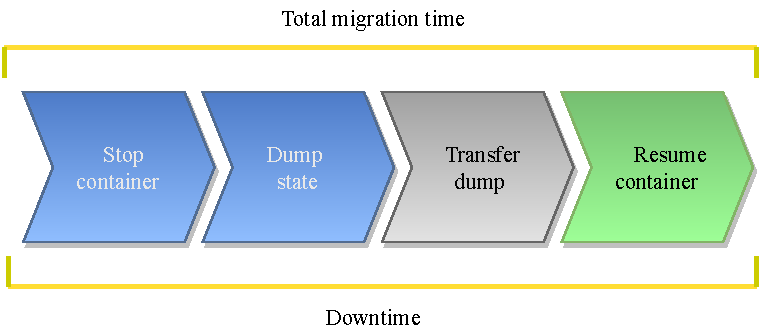
\includegraphics[scale=1]{migration_a_froid.pdf}
      \caption{La migration à froid \cite{puliafito2019}}
      \label{fig:migration_a_froid}
      \end{figure}
      \item \emph{La migration à chaud}: Contrairement à la migration à froid, les pages de mémoire de l'instance seront conservées et copiées vers l'hôte de destination pendant son exécution. Après quoi il reprend son exécution sur l'hôte de destination. On distingue trois sous-catégories de migration à chaud:
        \begin{enumerate}
          \item La migration avec pré-copie.
          \item La migration avec post-copie.
          \item La migration hybride.
        \end{enumerate}
      \end{enumerate}
\end{description}
\textbf{La migration avec pré-copie (méthode itérative)}: Dans ce cas, toutes les pages sont transférées au serveur de destination avant de geler le container. Mais quand les processus continuent leur exécution normale, les pages peuvent être modifiées et les pages transférées peuvent devenir obsolètes. C'est pourquoi les pages doivent être transférées itérativement. Sur la première étape, toutes les pages sont marquées d'un drapeau propre (clean flag) et transférées sur le serveur de destination [46]. Certaines pages peuvent être modifiées pendant ce processus, et l'indicateur propre sera supprimé dans ce cas. Sur la deuxième étape, seules les pages modifiées sont transférées vers le serveur de destination (voir Figure \ref{fig:migration_avec_precopie1}). La figure \ref{fig:migration_avec_precopie2} montre le séquencement des opérations de cette migration.\par
\begin{figure}[H]
\centering
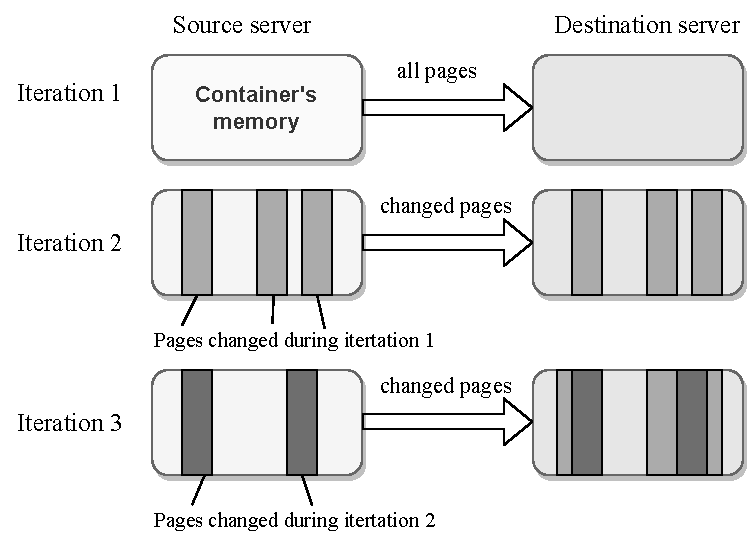
\includegraphics[scale=1]{iterative_migration.pdf}
\caption{Itérations de la migration avec pré-copie \cite{mirkin2008}}
\label{fig:migration_avec_precopie1}
\end{figure}
\begin{figure}[H]
\centering
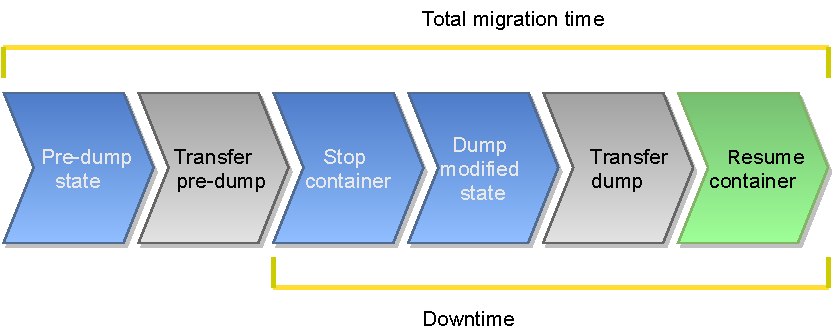
\includegraphics[scale=1]{migration_avec_precopie.pdf}
\caption{La migration avec pré-copie \cite{puliafito2019}}
\label{fig:migration_avec_precopie2}
\end{figure}
\textbf{La migration avec post-copie (fainéante)}: Par opposition à la technique précédente, toutes les pages mémoire allouées par les processus sont marquées d'un drapeau spécial, qui est effacé si une page est modifiée. Après cela, un conteneur peut être gelé et son état peut être sauvegardé, mais dans ce cas, seules les pages sans cet indicateur sont stockées. Cela permet de réduire la taille d'un fichier de vidage (dump). Puis au besoin, la machine destination génère des demandes de pages défectueuses (page-in swap), auxquelles la machine source répond en envoyant ces pages (à l'aide du daemon “page-out”), puis ces pages sont chargées en mémoire sur le serveur de destination (voir Figure \ref{fig:migration_avec_postcopie1}). C'est pour cette raison qu'elle est appelée migration fainéante. La figure \ref{fig:migration_avec_postcopie2} donne le schéma global de cette migration.\par
\begin{figure}[H]
\centering
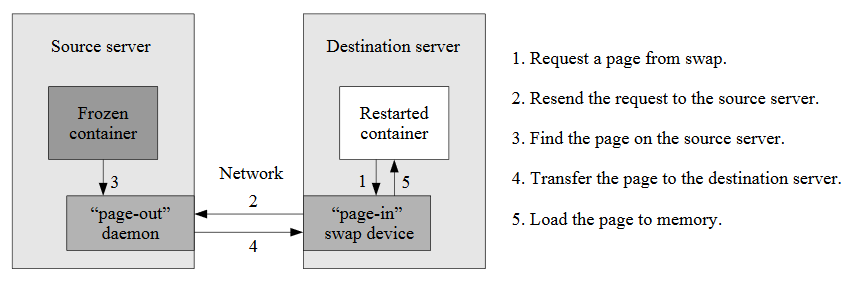
\includegraphics[scale=0.7]{lazy_migration.png}
\caption{Envoi des pages défectueuses \cite{mirkin2008}}
\label{fig:migration_avec_postcopie1}
\end{figure}
\begin{figure}[H]
\centering
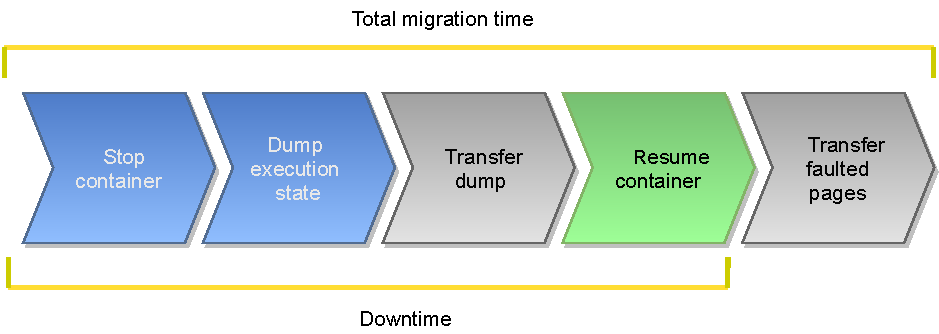
\includegraphics[scale=1]{migration_avec_postcopie.pdf}
\caption{La migration avec post-copie \cite{puliafito2019}}
\label{fig:migration_avec_postcopie2}
\end{figure}
\textbf{La migration hybride}: Les premières étapes coïncident avec celles de la migration avec pré-copie, une seule phase de pré-copie est effectuée avant la phase de post-copie,de cette manière l'hôte cible dispose déjà de toute la mémoire, seules les pages sales devront être transférées en post-copie. Une fois la mémoire copiée, le conteneur source est arrêté, et le conteneur destination est lancé sur l'hôte cible et la phase de post-copie commence \cite{wikimigration} (voir Figure \ref{fig:migration_hybride}).
\begin{figure}[H]
\centering
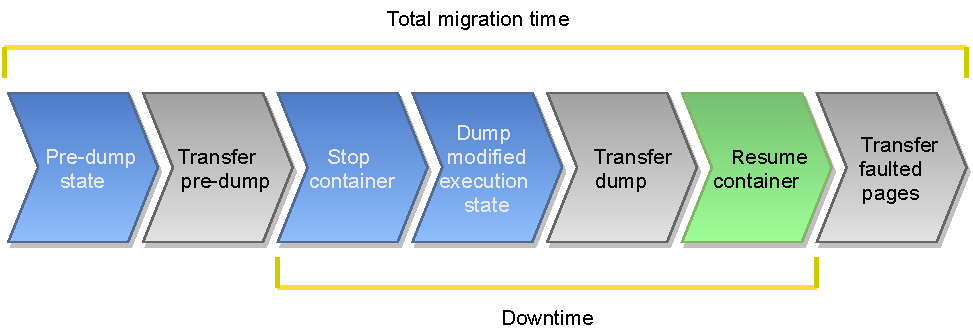
\includegraphics[scale=1]{migration-hybride.pdf}
\caption{La migration hybride \cite{puliafito2019}}
\label{fig:migration_hybride}
\end{figure}

\subsection{Taxonomie, Travaux réalisés}
Les travaux réalisés dans le domaine de virtualisation et migration de ressources virtuelles ont été classifiés selon la littérature en trois catégories selon l'objectif à optimiser \cite{rejiba2019}.
\begin{itemize}
  \item \emph{Optimisation du coût de la migration} : Visant soit à réduire les migrations coûteuses ou à trouver des compromis de coût de migration. Les processus de décision markovien constituent l'une des approches les plus utilisées pour modéliser le compromis de migration. Plus récemment, les efforts se sont progressivement déplacés vers la résolution du problème MDP en utilisant des approches apprentissage approfondi, qui ne nécessitent pas de connaissances préalables sur la dynamique de l'environnement MDP.
  \item \emph{Optimisation du temps de migration} : Les optimisations de migration focalisées sur l'axe du temps peuvent être divisées en optimisations proposées au niveau de la technologie de virtualisation et optimisations résultant de la prise d'actions proactives.
  \item \emph{Optimisation du taux d'erreur de la migration} : Les recherches sur ce sujet viennent exclusivement du domaine du cloud véhiculaire, à cause de la dynamicité le caractérisant, et qui peut potentiellement troubler le taux de succès de la migration. Ici, des techniques d'intelligence artificielle sont employées pour prédire la durée de disponibilité d'un véhicule dans une zone de couverture. Des protocoles de communication plus adaptés (comme le V2V) ont été aussi proposés.
\end{itemize}

%------------------------------------------------------------
\section{Gestion des ressources dans les environnements Fog Computing}
Contrairement au \emph{Cloud}, les ressources du \emph{Fog} sont : 
\begin{itemize}
  \item limitées en termes de performance et d'énergie - La plupart des noeuds \emph{Fog} possèdent généralement une  puissance de calcul ainsi que des ressources énergétiques limitées, dues principalement au fait que ces derniers sont constitués généralement des équipements d'interconnexion qui composent le réseau.
  \item hétérogènes - aussi bien sur le plan matériel, tel que différentes architectures de processeur, que sur le plan logiciel tel que différents systèmes d'exploitation.
  \item sujets à des défaillances - Les nœuds \emph{Fog} sont très susceptibles de subir des anomalies tels que des pannes de courant ou des défauts de capacité qui empêchent l'exécution des applications affectée à eux.
\end{itemize}
Dans de telles conditions, une gestion optimale des ressources est indispensable pour faire du \emph{Fog computing} une réalité. Ce qui fait de la gestion de ressource l'un des principaux défis du paradigme.

\subsection{Définition}
Selon \cite{red2020}, la gestion de ressources dans les environnements \emph{Fog} désigne \og{}les opérations administratives telles que le déploiement, la virtualisation et la surveillance des nœuds \emph{Fog} qui favorise les services d'infrastructure et de plate-forme basés sur le \emph{Fog}. De plus, la gestion des ressources du \emph{Fog} réalise l'équilibrage de charge, l'approvisionnement dynamique et la mise à l'échelle automatique pour assurer disponibilité du service et multi-location\fg{}.

\subsection{Dimensions du problème}
Le problème de la gestion des ressources dans les environnements \emph{Fog} est un problème complexe. Il ne peut donc pas être considéré comme étant un seul problème, mais plusieurs problèmes suivant plusieurs aspects \cite{mos2019}. Le problème peut être vu suivant  6 axes principaux que sont : le placement d'application, l'ordonnancement des tâches, le déchargement des tâches, l'équilibrage de charges, l'allocation de ressources ainsi que l'approvisionnement en ressources.
\begin{figure}[H]
  \centering
  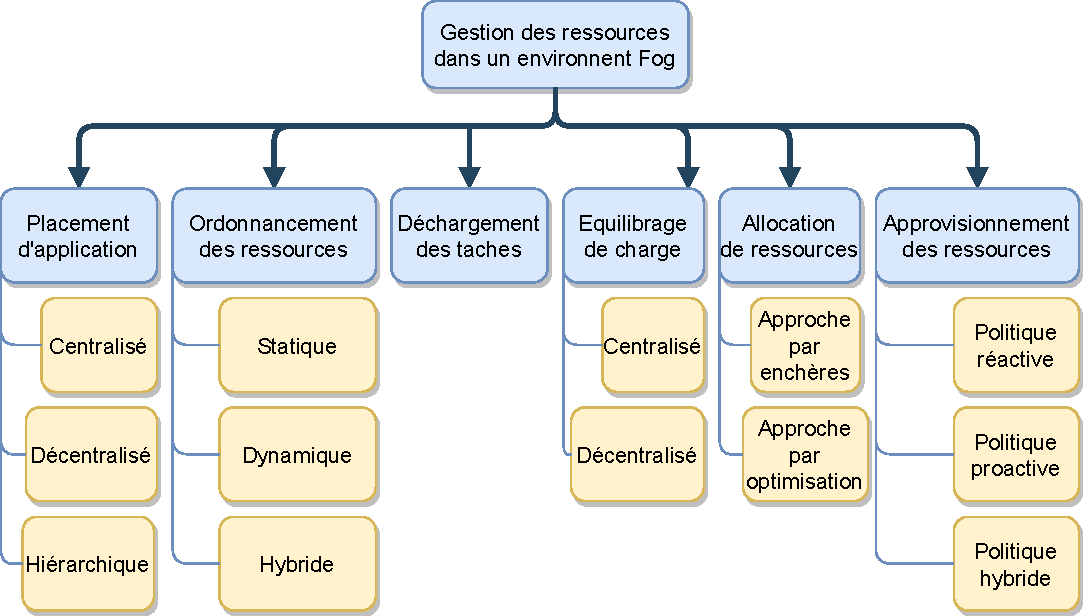
\includegraphics[scale=0.8]{organigrame_gestion_de_ressources.pdf}
  \caption{Organigramme qui illustre les domaines de gestion de ressource ainsi que leurs approches}
  \label{fig:organigrame_de_gestion_de_ressources}
\end{figure}

\subsubsection{Placement d'application}
Le problème de placement d'application désigne le problème de trouver une manière d'associer un service \emph{IoT} aux nœuds \emph{Fog} répondant aux exigences de la Qualité de service (QdS), tout en essayant de maximiser l'utilisation des différents nœuds .\\
D'une manière plus formelle soit $S$ un service \emph{IoT} avec des exigences de QdS $Q$, et soit $N$ l'ensemble des noeuds \emph{Fog}.\\
Une solution au problème de placement d'application consiste à associer au service $S$ un nœud \emph{Fog} $N_{i}$ de $N$ satisfaisant les exigences de QdS $Q$, tout en optimisant un ensemble de fonctions objectives $O$.\\
Il convient de préciser que les solutions peuvent être des relations multivaluées \emph{i.e.} un service \emph{IoT} peut être placé sur un ou plusieurs nœuds et réciproquement, un nœud peut héberger un ou plusieurs services.\par
Les approches basées sur la gestion de courtier “Broker” peuvent être organisées en 3 catégories que sont : l'approche centralisée, décentralisée et hiérarchique.
\begin{itemize}
  \item Dans l'approche centralisée, le broker nécessite d'avoir une vision globale de tout l'environnement \emph{Fog} afin de prendre des décisions d'optimisation pour l'ensemble du système. Cette approche ne garantit pas une optimisation efficace due à la difficulté d'obtenir toutes les informations de toutes les entités du \emph{Fog}, ainsi qu'une mauvaise tolérance aux pannes dues à son architecture centralisée.
  \item Tandis que  l'approche décentralisée, elle consiste en un ensemble d'optimisation locale ce qui la rend très intéressante en termes de scalabilité.
  \item Quant à l'approche hiérarchique, l'idée est  de relier et de coordonner les différents gestionnaires locaux afin qu'il puisse collaborer entre eux et ainsi bénéficier des avantages des deux premières approches. 
\end{itemize}

\subsubsection{Planification des ressources :}
Dans les environnements \emph{Fog}, un service \emph{IoT} peut être placé sur plusieurs nœuds, et chaque service peut être divisé en plusieurs sous-services.\\ 
Soit un ensemble de sous-services $S=\{S_{1},...,S_{n}\}$ (avec de différentes exigences en termes de QdS) placer sur un ensemble de nœuds $N=\{N_{1},...,N_{m}\}$ (ayant différentes capacités de traitement).\\
La planification de ressource consiste à trouver une affectation optimale des différents sous-services $S_{i}$ aux différents nœuds $N_{j}$ suivant les objectifs considérés par la politique d'ordonnancement (par exemple, minimiser le temps d'exécution).\\
Parmi les approches utilisées dans l'ordonnancement des ressources, les approches : 
\begin{itemize}
  \item \emph{Statique :} Dans cette approche, l'attribution des nœuds au différent sous-service s'effectue d'une manière statique i.e, la décision est déjà prise avant même que la demande ne soit soumise, ce qui présuppose une connaissance au préalable de toutes les informations nécessaires des différentes demandes.
  \item \emph{Dynamique :} contrairement à la précédente, le processus d'attribution  n'est pas fixé au préalable, les décisions sont prises une fois les demandes formulées.
  \item \emph{Hybride :} elle consiste en une combinaison des deux approches précédentes afin de répondre à la diversité des types d'application. 
\end{itemize}

\subsubsection{Déchargement des tâches}
Le déchargement de tâches désigne le processus de transfert des tâches qui ne peuvent pas être exécutées en local pour manque de ressource vers des nœuds disposant des capacités nécessaires. Vu les ressources matérielle et énergétique limitées dont disposent les appareils \emph{IoT}, il est souvent nécessaire de recourir à des entités externes telles que le \emph{Fog} ou le \emph{Cloud} afin d'exécuter des tâches gourmandes en ressource telle que des calculs graphiques, réalité augmentée, etc.\\
Le déchargement de tâche dépend principalement de trois composants que sont :
\begin{itemize}
  \item \emph{les appareils IoT:} dont le rôle est de spécifier comment les applications doivent être partitionnées, ensuite de déterminer quelle partie doit être exécutée en local, et quelle partie doit être déchargée.
  \item \emph{Les liaisons de communication:}  elles permettent d'assurer le transfert de tâche, et donc, la qualité des transferts dépend des capacités physiques des liaisons.
  \item \emph{Les nœuds Fog:} ces derniers disposent d'une capacité plus faible que le \emph{Cloud}, mais plus importante que les appareils \emph{IoT}.
\end{itemize}
Le déchargement de tâche peut se produire également afin d'assurer l'équilibrage de charge, minimiser la latence, efficacité énergétique, etc.

\subsubsection{Équilibrage de charge}
L'équilibrage de charge \cite{Ash2019} consiste à distribuer l'excédent de charges sur les différents nœuds \emph{Fog} suivant une certaine stratégie, afin d'assurer qu'aucun nœud \emph{Fog} ne soit en surcharge ou en sous-charge, améliorant ainsi les performances globales du système. Cependant, en réalité les mécanismes d'équilibrage de charge rencontrent de nombreux défis, principalement le problème de latence qui est due à la migration en continu des différents processus.\\
Les stratégies d'équilibrage sont implémentées suivant une architecture centralisée et décentralisée.
\begin{itemize}
  \item L'approche centralisée s'appuie sur un contrôleur central, nécessitant ainsi une connaissance globale et en temps réel de l'état des différents nœuds.
  Cette approche est donc difficile à implémenter dû à la difficulté de connaître en continu l'état des différents nœuds du système, mais aussi une tolérance faible aux pannes dues à son architecture centralisée.
  \item Quant à l'approche décentralisée, elle utilise un contrôleur décentralisé dont le rôle est de coordonner les différents contrôleurs locaux, ce qui assure une plus grande scalabilité.
\end{itemize}

\subsubsection{Allocation des ressources}
Le problème d'allocation des ressources dans les environnements \emph{Fog} peut être considéré comme un problème de double correspondance, car les serveurs \emph{Cloud} et les nœuds \emph{Fog} sont couplés pour les utilisateurs et l'utilisateur et les nœuds \emph{Fog} sont couplés pour les serveurs \emph{Cloud}. En d'autres termes, les utilisateurs doivent prendre en considération la relation entre les nœuds \emph{Fog} et les serveurs \emph{Cloud}, et les serveurs \emph{Cloud} doivent prendre en considération la relation entre les nœuds et les utilisateurs.\\ 
Les techniques d'allocation de ressource peuvent être classées en 2 principales méthodes :
\begin{itemize}
  \item \emph{Basé sur l'enchère “auction-based”:} les clients soumettent leurs demandes de ressources au broker avec un système de tarification des demandes, et les ressources se verront attribuer au plus offrant, en utilisant des mécanismes d'enchères calculés suivant diverses techniques mathématiques.
  \item \emph{Basée sur des techniques d'optimisation:} elle consiste à trouver la combinaison optimale (serveurs-cloud,noeud-fog,utilisateur) pour chaque utilisateur en effectuant des d'optimisation de fonctions objectives, telles que la minimisation du temps de réponse, la maximisation de la QdS, etc.
\end{itemize}

\subsubsection{Approvisionnement en ressources}
Dus aux fluctuations permanentes des charges de travail des différentes applications, les problèmes de sur-approvisionnement ou sous-approvisionnement de  ressources risquent de se poser.\\
Le problème de sur-approvisionnement consiste en une attribution d'une quantité de ressources supérieure à la charge de travail réelle d'une application. (Et réciproquement pour le problème de sous-approvisionnement).\\
Dans un environnement en constantes variations,  un modèle statique d'approvisionnement de ressources peut être problématique, il est par conséquent indispensable d'adopter une approche dynamique permettant ainsi l'adaptation en continu vis-à- vis des charges de travail.\\ 
Les stratégies d'approvisionnement dynamique sont classées en 3 types de politique :
\begin{itemize}
  \item \emph{Politique réactive:} elle consiste à répondre seulement aux différentes demandes, avec aucune tentative de prédiction des prochaines demandes.
  \item \emph{Politique proactive:} elle repose sur des techniques de prédiction permettant d'anticiper les prochaines évolutions des charges de travail et adapter les décisions en fonction.
  \item \emph{Politique hybride:} elle adopte par conséquent les deux précédentes politiques,  la politique réactive est souvent utilisée pour approvisionner des ressources à une nouvelle demande qui arrive dans le système, tandis que la politique proactive permet d'anticiper les prochaines évolutions de la demande. 
\end{itemize}

\subsection{Architectures proposées}
 Les différentes approches de gestion de ressources dans les environnements \emph{Fog} ont été classées suivant leurs architectures 3 types \cite{ch2019} :
 \begin{itemize}
  \item \emph{Les architectures basées sur flux de données (Data flow architectures):} Ces types d'architecture se basent sur le sens de transfert des charges de travail, par exemple les charges de travail peuvent être transférées de l'utilisateur au nœud \emph{Fog} ou des serveurs \emph{Cloud} vers les nœuds.
  \item \emph{Les architectures de contrôle (Control architectures):} Ces architectures sont basées sur la manière dont les ressources sont gérées au niveau du système, par exemple un contrôleur ou un algorithme central peut être utilisé pour gérer un ensemble de nœuds.
  \item \emph{L'architecture de location (Tenancy architecture):} cette architecture se base sur la capacité des différents nœuds à héberger plusieurs applications,  par exemple, une ou plusieurs applications peuvent s'exécuter sur un nœud \emph{Fog}.
\end{itemize}

\section{Conclusion}
Nous avons présenté dans ce chapitre les différents composants logiciels et matériels de l'architectures Fog, en l'occurrence les objets IoT, les VMs et les conteneurs ainsi que les contraintes de gestion de ressources imposées par ce paradigme.\par
Dans ce qui suit, nous nous intéresserons à la problèmatique de la gestion efficace de ressources disponibles dans les environnements Fog. Nous introduiserons dans ce cadre notre solution d'allocation de ressources, et l'algorithme sur lequel elle est basée.

\chapter{Solution d'allocation de ressources dans un environnement \emph{Fog Computing}: Stable Matching based Resources Allocation (SMRA)}
\thispagestyle{fancy}
\section{Introduction}
Nous avons vu à travers le chapitre précédent que le Fog Computing est caractérisé par l'hétérogénéité de ses composants à la fois matériel et applicatif. D'où le besoin d'une technique efficace permettant la gestion de l'allocation de ressources du Fog aux différentes applications l'utilisant.\par
Nous définirons dans ce chapitre les concepts sur lesquels repose note solution, et puis nous présenterons les algorithmes qui la composent et son scénario d'exécution nominal.


\section{Motivation}
Une bonne gestion de ressources permet d'accroître les performances globales du système, en réduisant le temps d'exécution des différentes applications, la latence, ainsi que les coûts énergétiques. Elle permet aussi d'exploiter au mieux les ressources matérielles disponibles, ce qui augmente le rendement et la rentabilité économique des différents équipements.\\ 
Par conséquent, le développement d'un bon modèle de gestion de ressource se révèle d'une importance capitale pour une exploitation efficace et rentable d'une infrastructure Fog.



\section{Problématique et article de référence}
Suite à l'étude des travaux qui traitent de l'amélioration et de l'optimisation de la gestion des ressources, on constate que le problème de planification des ressources est un problème central qui nécessite d'être investigué afin d'effectuer une gestion de ressources optimale. \\
Le problème consiste à concevoir un modèle de planification de ressources dynamique, efficace et évolutif, qui permet d'affecter les différentes demandes de ressources, effectuées par les appareils IoT, aux différents nœuds Fog d'une manière à optimiser au mieux certaines métriques liées aux coûts.\\
Pour la réalisation de ce travail, nous nous sommes inspirés d'un article publié traitant une problématique similaire \cite{jing2016}. \\
Dans ce travail, les auteurs s'intéressent au processus d'approvisionnement dans un environnement \emph{Cloud}, dans lequel ce processus peut être principalement décomposé en 3 étapes majeures à savoir : 
\begin{enumerate}
    \item L'identification des nœuds concernés (c.-à-d. les nœuds sous-utilisés ou sur-utilisés). 
    \item Sélection des VMs à migrer.
    \item Réallocation des VMs aux nœuds sous-utilisés.
\end{enumerate}
La partie qui nous intéresse est la troisième étape où ils proposent un mécanisme d'affectation de VMs aux nœuds adéquat, modélisé comme étant un problème de correspondance (matching problem).



\section{Contribution}



Dans ce travail, nous proposons une nouvelle technique d'allocation des nœuds d'un environnement Fog afin de mieux servir les requêtes générées par les objets \emph{IoT}. Cette technique, regroupé sous le sigle \emph{SMRA} pur \emph{Stable Matching based Resources Allocation}, se base sur une implémentation de l'algorithme de \emph{Gale-Shapley} \cite{gale-shapley}, et sera détaillé dans ce qui suit.\par



\subsubsection{Hypothèses}



Afin de pouvoir nous focaliser sur le problème de correspondance entre les demandes de services et les nœuds Fog, et à cause des limites de l'environnement de simulation, nous devons d'abord formuler certaines hypothèses sur la topologie physique de l'infrastructure Fog.\\



\begin{itemize}
    \item La topologie est statique durant l'exploitation: une fois la solution implémentée, la topologie ne subit pas de modification.
    \item La topologie suit une organisation matricielle: les nœuds Fog sont organisés en des niveaux bien distincts avec le même nombre de nœuds dans chaque niveau.
    \item La topologie est maillée entre les niveaux: chaque nœud Fog du cluster est relié physiquement à tous les nœuds du niveau supérieur.
    \item Chaque nœud à une connaissance de tous ses nœuds parents et ses nœuds enfants (c.-à-d. respectivement les nœuds du niveau supérieur et les nœuds du niveau inférieur)
    \item Dans ce modèle, nous disposons au minimum de trois types de requêtes qui sont : \\
          \begin{itemize}
             \item La requête \emph{demande}, qui correspond à une demande de services émise par les appareils IoT, elle comporte tous les détails de la demande.
             \item la requête \emph{résultat}, qui est généré après l'exécution d'une demande de service, elle est émise à destination de l'objet \emph{IoT} émetteur.
             \item La requête \emph{jeton}, qui représente le jeton circulant entre les différents nœuds passerelle suivant la politique du tourniquet (round-robin).
          \end{itemize}
\end{itemize}




\subsection{Architecture SMRA}



SMRA se décompose en 4 aspects interdépendants que nous détaillons par la suite:



\begin{description}
  \item[La clusterisation (Clusterization):] en regroupant les nœuds Fog dans des groupes (Cluster) de par leur proximité géographique.
  \item[le profilage (Profiling):] en attribuant différents profiles ou rôles aux différents nœuds d'un cluster.
  \item[Le traitement par lot (Batch processing):] les demandes sont regroupées et traitées par lot selon leurs ordres d'arrivée.
  \item[La correspondance (matching):] le processus d'association et de redirection des demandes vers les nœuds Fog adéquats.
\end{description}
\newpage
\subsection{Clusterisation (Clusterization)}



Comme vu précédemment, une infrastructure \emph{Fog} classique est décomposée de 3 couches superposées qui sont (voir Figure \ref{fig:Topologie_generale_de_linfrastructure}) :



\begin{itemize}
    \item \emph{La couche IoT}, qui représente l'ensemble des objets \emph{IoT} qui effectue des demandes de service.
    \item \emph{La couche Fog}, qui représente l'ensemble des nœuds \emph{Fog} se trouvant à l'intermédiaire entre les objets \emph{IoT} et le \emph{cloud}.
    \item \emph{La couche Cloud} qui représente l'infrastructure Cloud traditionnelle.
\end{itemize}



\begin{figure}[H]
    \centering
    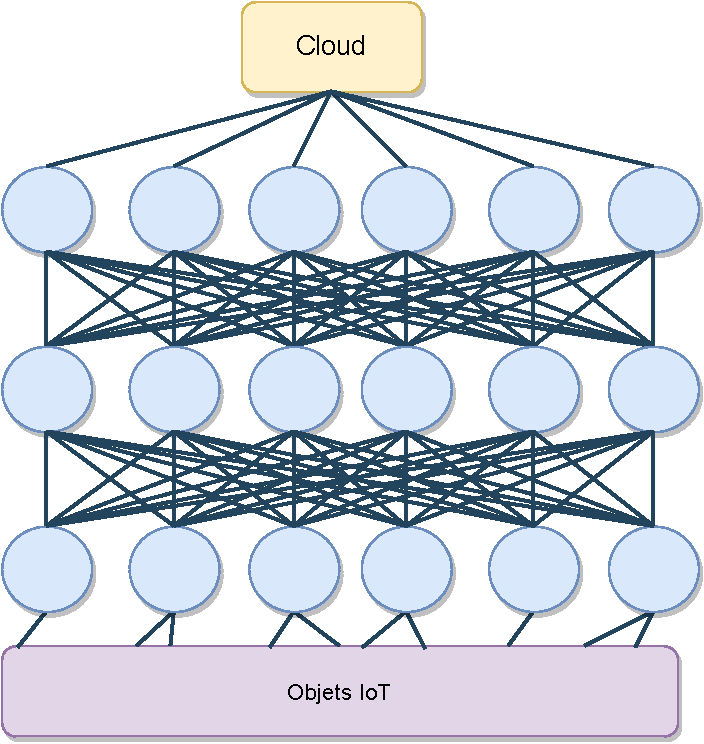
\includegraphics[scale=0.9]{Topologie_générale_de_l'infrastructure.pdf}
    \caption{Schémas représentant une architecture Fog traditionnelle}
    \label{fig:Topologie_generale_de_linfrastructure}
\end{figure}



\par SMRA commence par découper verticalement la couche \emph{Fog} de l'infrastructure en un ensemble de clusters\footnote{Nous discutons des critères de scalabilité verticale et horizontale du cluster dans le chapitre suivant, où nous montrons les résultats obtenus par rapport à différentes dimensions du cluster.} (voir Figure \ref{fig:Infrastructure_fog_repartie_en_cluster}) , c.-à-d. chaque cluster regroupe un ensemble de nœuds \emph{Fog} inter-connecté.



\begin{figure}[H]
    \centering
    \includegraphics[scale=0.9]{ShémaCluster.pdf}
    \caption{Schéma représentant une architecture \emph{Fog} répartie en clusters}
    \label{fig:Infrastructure_fog_repartie_en_cluster}
\end{figure}



\subsection{Profilage (Profiling)}
Une fois l'infrastructure est répartie en cluster, SMRA attribue des profiles aux noeuds constituant le cluster (voir Figure \ref{fig:profilage}) en définissons deux profile que sont :
\begin{itemize}
  \item Le profil \emph{Noeud Passerelles} (en rouge) : qui est adoptée par les noeuds du niveau connecté directement à la couche \emph{IoT}.
  \item Le profil \emph{Noeud Fog} (en bleu) : qui est attribué aux noeuds des niveaux intermédiaires restants entre la couche des nœuds passerelles et le \emph{cloud}. 
\end{itemize}



\begin{figure}[H]
  \centering
  \includegraphics[scale=0.9]{ShémaProfile.pdf}
  \caption{Schéma représentant les profils des noeuds au sein d'un cluster}
  \label{fig:profilage}
\end{figure}



\subsection{Scénario}
Ce scénario s'applique pour un cluster, puisque les clusters sont indépendants, il suffit par la suite de généraliser ce fonctionnement à l'ensemble des clusters défini par l'infrastructure.\par
Les nœuds passerelles du cluster, reçoivent des demandes de services des différents appareils IoT. Chaque nœud préserve ses demandes dans une file en attendant leur correspondance puis leur envoi à leur destination.\par
Nous définissons un jeton circulant d'un nœud passerelle à un autre suivant la politique du tourniquet (round robin). Si un nœud passerelle possède le jeton à la réception alors il effectue une correspondance des demandes qui se trouve dans sa file d'attente avec les nœuds \emph{Fog} du cluster, puis il envoie chaque demande au nœud \emph{Fog} correspondant, et  renvoie le jeton au prochain nœud passerelle et ainsi de suite (voir Figure \ref{fig:Organigrame_scénario_globale}).



\begin{figure}[H]
  \centering
  \includegraphics[]{Organigramme-scénario-globale.pdf}
  \caption{Organigramme du scénario d'exécution du SMRA}
  \label{fig:Organigrame_scénario_globale}
\end{figure}



\subsection{Description algorithmique du scénario}



SMRA est conçu suivant le paradigme événementiel, c.-à-d. une approche algorithmique basée sur la notion d'événement, où on cherche à associer à chaque événement une procédure à exécuter appelée “Routine”.   
SMRA comporte 2 routines principales qui sont :
\begin{itemize}
    \item \emph{La Routine associée aux nœuds passerelles}
    \item \emph{La Routine associée au nœud Fog}
\end{itemize}



\subsubsection{Routine associée aux nœuds passerelles}
Cette routine est exécutée au niveau des nœuds passerelles à chaque fois qu'une requête est reçue.
Le pseudo-code de cette routine est le suivant :\\
\begin{algorithm}[H]
  \KwData{ListeDemandes, ListeNoeuds}
  \eIf{Requête reçue est de type jeton}
  {  
    \emph{// appeler la  procédure Correspondance.}\\
    correspondance(fileDemandes, listeNoeuds);\\
    \emph{// puis on effectue le routage des demandes.}\\
    \ForEach{Demande $D_i \in fileDemandes$}
    {
      \eIf{listeParents.contient($D_i$.destination)}
      {
        envoyer(demande, $D_i$.destination);
      }
      {
        envoyer(demande, NoeudPèreParDéfaut);\\
        \emph{// on met à jour le nœud par défaut à chaque fois afin d'équilibrer la charge entre les différentes liaisons.}\\
        NoeudPèreParDéfaut $\gets$ prochainNoeudParent();\\
      }
    }
  }
  {
    \eIf{Requête reçue est de type résultat}
    {
      \emph{// envoyer le résultat à l'appareil IoT concerné.}\\
      envoyer(resultat, resultat.destination);
    }
    {
      \emph{// la requête est par conséquent de type demande.}\\
      enfiler(fileDemandes, Demande);
    }
  }
  \caption{Routine associée aux nœuds passerelles}
\end{algorithm}
\\
\paragraph{Procédure de correspondance :}
Pour l'implémentation de cette procédure, nous avons opté pour l'utilisation de l'algorithme de Gale-Shapley \cite{gale-shapley}, qui est un algorithme conçu pour résoudre le problème des mariages stables.\\
Il présente des propriétés intéressantes qui sont :
\begin{itemize}
  \item De bonne performance due à sa complexité quadratique ($\mathcal{O}(n^2)$).
    \item Convergence: toute demande sera associée à un nœud à la fin de l'exécution.
    \item Les couples (demande,nœud) résultant de cet algorithme sont stables (voir Annexe).
    \item La configuration résultante est optimale en comparaison à toutes les autres solutions stables \cite{gale-shapley}.
\end{itemize} \\
Cet algorithme nécessite la définition d'une relation de préférence, que nous nommerons "Relation d'adéquation" ou RA qui est associée à chaque demande et à chaque nœud:\\
Pour ce faire, nous définissons une distance entre la demande et le nœud, qui est calculé de la manière suivante :
\\ \\
\begin{minipage}[t]{0.4\textwidth}
\begin{flushleft}
    \begin{tabular}{| c | p{4cm}|}
    \hline
    Symbole & Définition \\
    \hline
    $C_u$ & MIPS\footnote{million d'instructions par seconde} utilisé \\ 
    \hline
    $C_{dem}$ & MIPS exigés par le service à exécuter \\
    \hline
    $C_fd$ & MIPS total du nœud \\
    \hline
    $C_r$ & MIPS disponible \\
    \hline
    \end{tabular}
\end{flushleft}
\end{minipage}
%
\begin{minipage}[th]{0.4\textwidth}
\begin{flushright} 
\begin{center}
    $$Distance =\left \lbrace 
    \begin{array}{ll}
        \frac{C_u + Cdem}{C_fd}/ & \mbox{si $C_r > C_{dem}$}\\
        -1 & \mbox{sinon}
    \end{array}
\right.$$
\end{center}
\end{flushright}
\end{minipage}
\\ \\ \\
La relation d'adéquation est définie par la distance minimale entre le nœud et la demande.\\
Autrement dit, soit $D=\{D_1,D_2,..,D_n\}$ un ensemble de demandes, et soit $N=\{N_1,N_2,..,N_n\}$.\\
On dit que le nœud $N_j$ est le mieux adéquat à la demande $D_i$ ssi : \\
$Distance(D_i,N_j) = Min (Distance(D_i,N_m)), \forall m \in \{1,..,n\}$. \\
\textbf{Pseudo-code de la procédure :}\\
\begin{algorithm}[H]
  \KwData{ListeDemandes, ListeNoeuds}
  \emph{// initialisation de toutes les demandes à une destination null.}\\
  \ForEach{Demande $D_i \in ListeDemandes$}
  {
    $D_i$.destination $\gets$ null;\\
  }
  \While{$\exists$ une\ demande\ $d$\ non\ affectée\ qui\ peut\ se\ proposer\ à\ un\ nœud}
  {
    %n $\gets$ le\ nœud\ le\ mieux\ adéquat\ à\ $d$\ parmi\ la\ liste\ des\ nœuds\ auquel\ $d$\ ne\ s'est\ pas\ déjà\ proposé;\\
    n $\gets$ le\ nœud\ le\ mieux\ adéquat\ à\ $d$\ telque\ $d$\ \notin\ $nœud.demandesRejetées$;\\
    \eIf{$n$ = null}
    {
      \emph{// si aucun nœud ne peut traiter la demande, elle est déléguée au cloud.}\\
      d.destination $\gets$ cloud;\\
      envoyerVersCloud(d);\\
    }
    {
      \eIf{$n$ est libre}
      {
        d.destination $\gets$ n;\\
      }
      {
        \emph{// si le nœud n'est pas libre et que $d$ est plus adéquate que la demande associée à n.}\\
        \eIf{distance(n,n.demande) > distance(n,d)}
        {
          \emph{// la destination de la demande associée à n est remise à null pour qu'elle soit retraiter.}\\
          n.demande.destination $\gets$ null;\\
          \emph{// puis elle est ajoutée aux demandes rejetées par le nœud pour qu'elle ne puisse pas se reproposer.}  \\
          n.demandesRejetées.ajouter(n.demande);\\
          \emph{// la demande associée à n est remplacée par d.}\\
          n.demande $\gets$ d;\\
          d.destination $\gets$ n;\\
        }
        {
          \emph{// la demande d a été rejetée par le nœud donc elle ne peut plus se reproposer.}\\
          n.demandesRejetées.ajouter(d);\\
        }
      }
    }
  }
  \caption{Procédure de correspondance}
\end{algorithm}



\subsubsection{Routine associée au nœud Fog :}
Cette routine est exécutée au niveau des nœuds Fog à chaque fois qu'une requête est reçue.\\
\textbf{Pseudo-code de la routine :}\\
\begin{algorithm}[H]
  %\KwData{this text}
  %\KwResult{how to write algorithm with \LaTeX2e }
  \eIf{Requête reçue est de type demande}
  {  
    \eIf{demande.destination correspond au nœud lui-même}
    { 
      \emph{// la destination du résultat et la source de la demande.}\\
      resultat $\gets$ executer(demande);\\
      \emph{// puis effectuer le routage du résultat.}\\
      \eIf{listeEnfants.contient(resultat.destination)}
      {
        envoyer(resultat, resultat.destination);\\
      }
      {
        envoyer(resultat, NoeudFilsParDefaut);\\
        NoeudFilsParDéfaut $\gets$ prochainNoeudFils();\\
      }
    }
    {  
      \emph{// le nœud en question n'est pas la destination.}\\
      \eIf{listeParents.contient(demande.destination)}
      {
        envoyer(demande, demande.destination);\\
      }
      {
        envoyer(demande,NoeudPèreParDéfaut);\\
        NoeudPereParDéfaut $\gets$ prochainNoeudParent();\\
      }
    }
  }
  {
    \emph{// la requête reçue est par conséquent une requête résultat.}\\
    \eIf{listeEnfants.contient(resultat.destination)}
    {
      envoyer(resultat, resultat.destination);\\
    }
    {
      envoyer(resultat, NoeudFilsParDefaut);\\
      NoeudFilsParDéfaut $\gets$ prochainNoeudFils();\\
    }
  }
  \caption{Routine associée aux nœuds passerelles}
\end{algorithm}



\section{Conclusion}
Dans ce chapitre, nous avons présenté notre solution en introduisant les entités interagissantes de notre environnement tout en formulant certaines hypothèses sur ce dernier. Nous avons décrit aussi le scénario nominal d'exécution et nous avons détaillé les algorithmes exploités à chaque niveau.\par
 Dans le prochain chapitre, nous passerons à l'étape d'implémentation de la solution sur une plateforme de simulation d'environnement Fog, et nous finirons par une discussion des résultats obtenus.
\chapter{Implémentation et résultats}
\thispagestyle{empty}
\newpage
\section{Introduction}
Dans le chapitre précédent, nous avons présenté toute la théorie mise en place pour la conception de notre solution de planification de ressources relative à la gestion des ressources dans les environnements Fog. Pour cela, nous avons besoin d'outils nous permettant la quantification des performances et la production de résultat, afin de pouvoir effectuer l'évaluation.\\
Ce chapitre commence par donner un aperçu global sur les différents outils utilisés pour mener à bien la simulation de cette solution, ainsi que les différents éléments ajoutés au simulateur. Enfin nous présentons les résultats en les comparant avec les résultats des différentes politiques gestion classique que sont les politiques : “First fit”, "Best Fit" et "Worst fit".\\

\section{Outil de développement}
Afin de pouvoir simuler la solution proposée, nous avons opté pour le simulateur “IFogSim”. En effet ce dernier opère suivant le paradigme événementiel, ce qui s'accorde parfaitement avec notre solution qui use du même concept. Développé exclusivement en java, IFogSim nous permet de mesurer l'impact technique résultant de la gestion en nous fournissant des données concernant la consommation d'énergie, les délais d'exécution et l'état du réseau.

\subsection{Langage JAVA}
Java est une technologie initialement développée par la société “Sun Microsystems” en 1995, cette dernière s'est vue rachetée par la suite par la société Oracle en 2009. Java fait office à la fois de langage de programmation orienté objet, mais aussi de machine virtuelle qui permet au langage Java d'être multiplateforme. La technologie java bénéficie d'une grande popularité dû aux avantages considérables proposés par cette dernière parmi lesquels :
\begin{itemize}
    \item La portabilité : i.e la capacité du même code java à s'exécuter sur plusieurs systèmes d'exploitation.
    %\item Popularité
    \item Richesses des bibliothèques disponibles
    \item Gratuité 
\end{itemize}

\subsection{L'outil IFogSim}
IFogSim est un outil de modélisation d'environnements Cloud-Fog-IoT créé par
Harshit Gupta (chef de projet) au Georgia Institute of Technology, Atlanta, GA, USA dans l'objectif de simuler l'impact des différentes techniques du management des ressources sur les environnements Fog. IFogSim mesure l'impact d'une politique sur un système par sa latence, l'utilisation de la bande passante, la consommation d'énergie et l'utilisation des ressources des nœuds. IFogSim a été conçu en tant qu'extension à l'outil CloudSim, qui est un simulateur Open Source d'applications Cloud développé en Java. IFogSim est donc lui aussi Open Source et programmé en Java .

\subsection{Architecture de l'IFogSim}
L'iFogSim est composé de 3 composants principaux, à savoir : 
\begin{itemize}
    \item Les composants physiques.
    \item Les composants logiques.
    \item Les composants de gestion.
\end{itemize}

\subsubsection{Composants physiques}
Les composants physiques incluent le cloud, les nœuds Fog et les objets, qui sont organisés dans un ordre hiérarchique. Les nœuds Fog de niveau inférieur sont directement connectés aux capteurs et actionneurs associés. Les nœuds Fog agissent comme des centres de traitement de données en offrant de la mémoire et de la puissance de calcul. Chaque nœud Fog est créé avec une puissance de calcul et des attributs de consommation d'énergie spécifique (puissance occupée et inactive), qui reflètent ses capacités et son efficacité énergétique. Les capteurs génèrent des tuples qui peuvent être appelés tâches dans le cloud computing. La création de tuples (tâches) est pilotée par les événements et l'intervalle entre la génération de deux tuples est régi par une distribution déterministe définie lors de la création des capteurs.

\subsubsection{Composants logiques}
Les modules d'application (AppModules) et les bords d'application (AppEdges) sont les composants logiques d'IFogSim. Dans IFogSim, une application est considérée comme une collection des modules interdépendants, ce qui améliore par conséquent le concept d'application distribuée. La dépendance entre deux modules est définie par les fonctionnalités d'AppEdges qui sont le flux de données logique entre deux modules d'application. Dans iFogSim, chaque module d'application (AppModule) traite un type particulier de tâche (tuple). La transmission de tuples entre deux modules d'application (AppModules) peut être périodique.

\subsubsection{Composants de gestion}
Les composants de gestion d'IFogSim sont représentés par le « Controller» et le «ModuleMapping». Selon les exigences des AppModules, l'objet ModuleMapping identifie les nœuds Fog associés à chaque AppModules. L'objet Controller lance les AppModules sur leurs nœuds Fog attribués en suivant les informations de placement fournies par l'objet ModuleMapping, et gère périodiquement les ressources des nœuds Fog. Une fois la simulation terminée, l'objet Controller collecte les résultats des coûts, de l'utilisation du réseau et de la consommation d'énergie pendant la période de simulation à partir des nœuds Fog.
\begin{figure}[H]
    \centering
    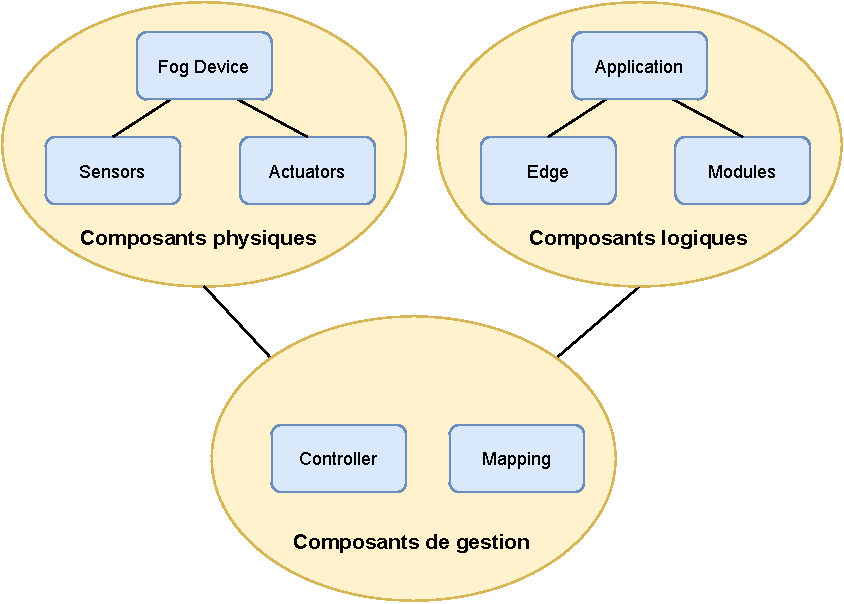
\includegraphics[]{Diagramme d'interaction.pdf}
    \caption{Diagramme représentant l'interaction des différents composants de l'IFogSim}
    % \label{fig:}
\end{figure}

\subsubsection{Description des classes principales}
Les principales classes de l'IFogSim sont les suivantes :
\begin{itemize}
    \item \textbf{\emph{FogDevice :}} Cette classe spécifie les caractéristiques matérielles des nœuds Fog et leurs connexions aux autres nœuds de la topologie. Les principaux attributs de cette classe sont la mémoire accessible, le processeur, la taille de stockage, la bande passante de la liaison montante et la liaison descendante. Les méthodes de cette classe définissent la manière dont les ressources d'un nœud Fog sont planifiées entre les modules qui s'exécutent sur cette application, ainsi que leur déploiement. Par défaut, chaque FogDevice ne peut avoir hiérarchiquement qu'un seul père.
    \item \textbf{\emph{Sensor :}}  les instances de la classe Sensor sont des entités qui agissent en tant que capteurs IoT tels que décrits dans l'architecture. La classe contient des attributs représentant les caractéristiques d'un capteur (son nom, le tuple d'émission et un paramètre qui représente les conditions d'émission du Tuple). La classe contient un attribut de référence au dispositif Fog auquel le capteur est connecté et la latence de connexion entre eux. 
    \item \textbf{\emph{Actuator  :}} -  Cette classe modélise un actionneur en définissant l'effet de l'actionnement et ses propriétés de connexion au réseau. La classe définit une méthode pour effectuer une action à l'arrivée d'un tuple à partir d'un module d'application. Un attribut de la classe fait référence à la passerelle à laquelle l'actionneur est connecté et à la latence de cette connexion.
    \item \textbf{\emph{Tuple :}} Les tuples forment l'unité fondamentale de communication entre les entités dans le réseau Fog. Il peut être soit une tâche, soit une donnée. Un tuple est caractérisé par son type, sa source et sa destination. Les attributs de la classe spécifient la puissance de calcul nécessaire à son traitement (mesuré en millions d'instructions (MI)) et la longueur des données encapsulées dans le tuple.
    \item \textbf{\emph{Application :}} Les instances de cette classe représentent les éléments qui composent une application. Pour chaque tuple entrant, une instance AppModule le traite et génère des tuples en sortie, qui sont envoyés aux modules suivants. Le nombre de tuples de sortie par tuple d'entrée est déterminé à l'aide d'un modèle de sélectivité, qui peut être basé sur une sélectivité fractionnaire ou un modèle éclaté.
    \begin{itemize}
        \item \textbf{\emph{AppEdge :}} Une instance AppEdge dénote la dépendance entre une paire de modules d'application. Chaque AppEdge est caractérisé par le type de tuple qu'il transporte, les exigences de traitement et la longueur des données encapsulées dans ces tuples. l'IFogSim prend en charge deux types d' AppEdge (périodique et événementiels). Les tuples dans les AppEdge périodiques sont émis à intervalles réguliers. Le tuple dans un AppEdge est basé sur un événement qui est envoyé lorsque le module source reçoit un tuple précis.
        \item \textbf{\emph{AppLoop :}} est une classe supplémentaire, utilisée pour spécifier les boucles de contrôle de processus qui intéressent l'utilisateur. Dans l'IFogSim, le développeur peut spécifier les boucles de contrôle pour mesurer la latence de bout en bout. Une instance AppLoop est fondamentalement une liste de modules à partir de l'origine de la boucle jusqu'au module où la boucle se termine.
    \end{itemize}
    \item \textbf{\emph{Config :}} Cette classe abstraite a pour but de contenir tous les paramètres qui affectent la simulation par exemple MAX\_SIMULATION\_TIME qui représente la durée de simulation.
    \item \textbf{\emph{Controller :}} cet objet se charge d'orchestrer la simulation. Concrètement, il sert à initialiser la topologie avant le début de la simulation, ainsi qu'à effectuer les traitements de fin de simulation (notamment afficher et exporter les résultats).
\end{itemize}
\begin{figure}[H]
    \centering
    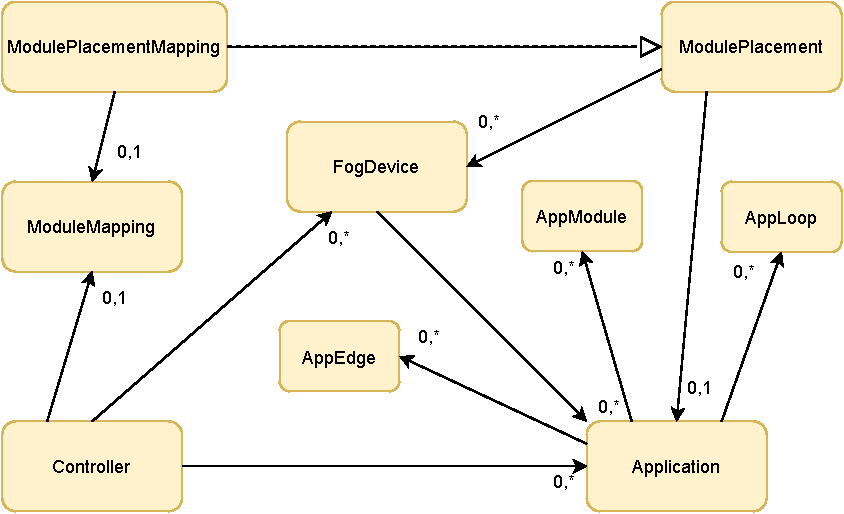
\includegraphics[]{DiagrammeDeRelation.pdf}
    \caption{Diagramme représentant les relations entre les principales classes de l'IFogSim}
    % \label{fig:}
\end{figure}

\section{Développement de la conception}
Afin de mettre en œuvre la conception proposée, nous allons ajouter de nouvelles classes nécessaires à l'implémentation de la solution, mais aussi la modification de certaines classes principales de l'IFogSim afin de l'adapter à nos besoins.\\
Les manipulations effectuées pour mettre en oeuvre cette solution sont énumérées ci-dessous : 
\begin{enumerate}
    \item \textbf{Création d'une classe ClusterFogDevice :} Cette classe représente un nœud Fog quelconque du cluster. Elle étend la classe prédéfinie FogDevice et comporte en plus les attributs suivant:
\begin{itemize}
    \item \textbf{parentsIds :} qui est une liste qui contient les identificateurs des nœuds se trouvant au niveau supérieur.
    \item \textbf{isNorthLinkBusyById :} qui est une liste de booléens où chaque élément indique si la liaison supérieure en question est occupée.
    \item \textbf{northTupleQueues :} qui est une liste de files d'attente de tuple qui associe à chaque liaison supérieure une file de tuples où seront stockés les tuples à envoyer sur cette liaison si cette dernière est occupée.
\end{itemize}
De plus, la méthode  processTupleArrival, qui est la méthode exécutée par le nœud à chaque arrivée d'un tuple, a été redéfinie afin d'implémenter la routine associée à un nœud Fog et qui est décrite dans la conception.
     \item \textbf{Création d'une classe GWFogDevice :} cette classe représente un nœud Fog passerelle, c.-à-d. le nœud connecté directement aux capteurs et aux actionneurs. Cette classe étend également la classe FogDevice, et ajoute les attributs suivants :
     \begin{itemize}
     \item \textbf{waitingQueue :} qui est une liste de tuples servant à stocker les demandes non encore affectées.
     \item \textbf{tupleToMatchedDevice :} est une liste contenant les tuples non affectés à un neud.
     \item \textbf{matchedTupleList :} qui est une liste comportant les tuples affectés à leurs nœuds respectifs.
     \item \textbf{gwDevices :} est une liste de GWFogDevice, contenant l'ensemble de nœuds passerelles.
     \item \textbf{isNorthLinkBusyById :} qui représente la même chose que dans la classe.
     \item \textbf{northTupleQueues :} elle représente également la même chose que celle mentionnée dans la classe ClusterFogDevice.
     \item \textbf{clusterFogDevicesIds :} qui représente la liste de tous les nœuds Fog du cluster.
     \end{itemize}
     \item \textbf{Création d'une classe MatchedTuple :} cette classe décrit les tuples une fois affectés à leurs nœuds respectifs. Elle représente un enrichissement de la classe Tuple par les attributs suivants :
     \begin{itemize}
         \item \textbf{destinationFogDeviceId :} qui contient l'identificateur du nœud de destination.
         \item \textbf{destModuleMips :} qui décrit les exigences de traitement du module de destination.
     \end{itemize}
\end{enumerate}
La même procédure à été effectueé pour implémenter les politiques concurrentes.

\section{Résultats et évaluation des performances :}
Afin de pouvoir juger des performances ainsi que l'ampleur des gains apportés par notre modèle de planification de ressources, nous évaluons les performances de cette solution en mesurant le délai d'exécution des applications, et le délai d'exécution des tuples. Puis nous comparons les résultats avec des modèles classiques implémentant les stratégies “FirstFit”,"BestFit","WorstFit".\par
Les nœuds \emph{Fog} ainsi que les demandes générées sont créés avec une certaine hétérogénéité permettant de mieux étudier la capacité de notre algorithme à faire correspondre une variété de demandes à des nœuds avec de différentes capacités matérielles.\par
Les résultats sont représentés par les graphes suivants (les résultats sont normalisés par rapport à la valeur maximale, donc sur une échelle de 0 à 1) :

\subsubsection{Scalabilité verticale}
Nous mesurons dans cette partie les performances du modèle par rapport à la variation du nombre de niveaux de la matrice \emph{Fog} précédemment définie.\par
Nous fixons dans cette expérience le nombre de nœudspar niveau à 5 nœuds.

\begin{figure}[H]
  \centering
  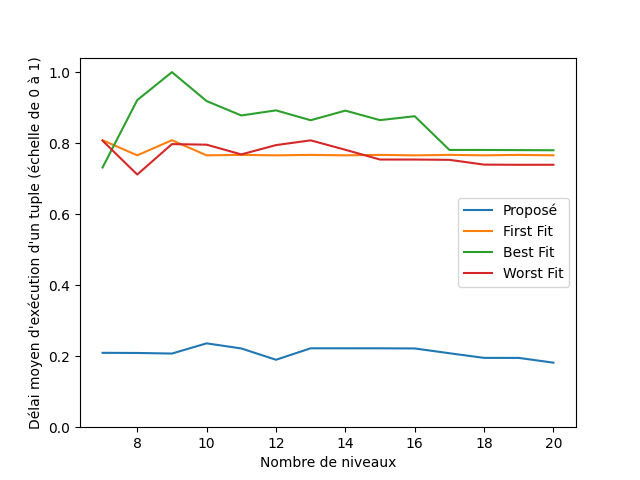
\includegraphics[]{resultats/tupleDelayV.png}
  \caption{Délai moyen d'exécution d'un tuple en fonction du nombre de niveaux}
  \label{fig:delai_tuple_vertical}
\end{figure}

\begin{figure}[H]
  \centering
  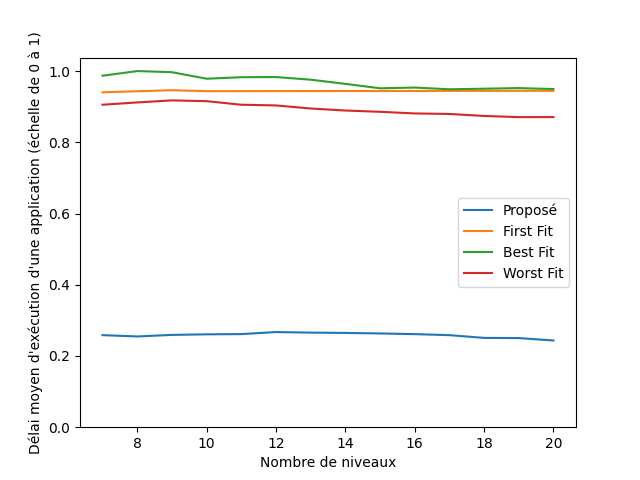
\includegraphics[]{resultats/loopDelayV.png}
  \caption{Délai moyen d'exécution d'une application en fonction du nombre de niveaux}
  \label{fig:delai_application_vertical}
\end{figure}

Les figures \ref{fig:delai_tuple_vertical} et \ref{fig:delai_application_vertical} montrent, respectivement, la variation du délai moyen de l'exécution d'un tuple (représentant une demande de service) et le délai d'exécution d'une application complète selon la nombre de niveaux de l'architecture.\par
Nous constatons une nette réduction du délai de traitement des tuples d'environ 75\%, en comparaison aux autres algorithmes de la simulation. Cette réduction se stabilise au-delà du seuil de 18 niveaux, où le nombre de niveaux n'influence plus cette métrique. De même pour le délai d'exécution d'une application, où nous pouvons constater l'impact de la réduction du temps de réponse des tuples individuels.

\subsubsection{Scalabilité horizontale}
Nous mesurons dans cette partie les performances du modèle par rapport à la variation du nombre de nœuds par niveau de la matrice \emph{Fog} précédemment définie.\par
Le nombre de nœuds par niveau influence le nombre de tuples générés par les objets IoT car chaque nœud passerelle est relié à un ensemble d’objets IoT. Ainsi l’augmentation du nombre de nœuds passerelle augmente aussi le nombre de demandes générées.\par
Nous fixons le nombre de niveaux à 10 niveaux.

\begin{figure}[H]
  \centering
  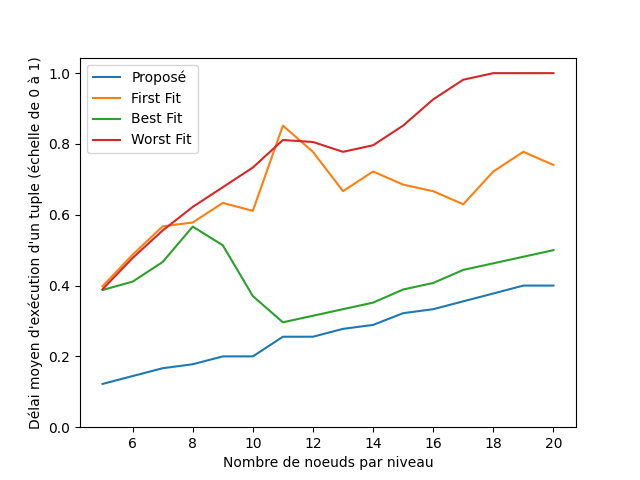
\includegraphics[]{resultats/tupleDelayH.png}
  \caption{Délai moyen d'exécution d'un tuple en fonction du nombre de nœuds par niveaux}
  \label{fig:delai_tuple_horizontal}
\end{figure}

\begin{figure}[H]
  \centering
  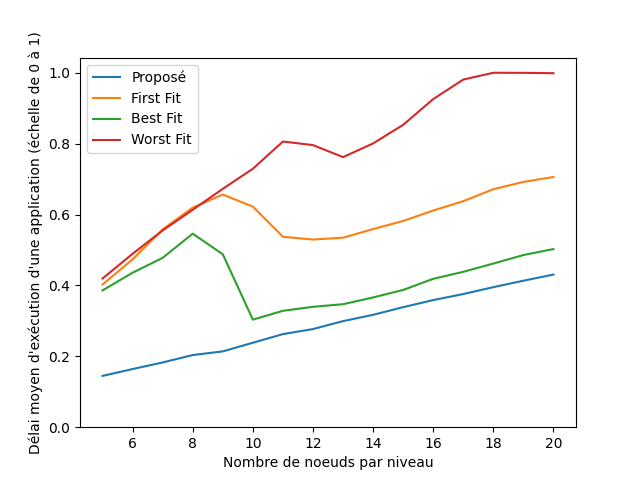
\includegraphics[]{resultats/loopDelayH.png}
  \caption{Délai moyen d'exécution d'une application en fonction du nombre de nœuds par niveau}
  \label{fig:delai_application_horizontal}
\end{figure}

Les figures \ref{fig:delai_tuple_horizontal} et \ref{fig:delai_application_horizontal} représentent, respectivement, la variation du délai de l'exécution d'un tuple et le délai d'exécution d'une application selon le nombre de nœuds par niveau.\par
La figure \ref{fig:delai_tuple_horizontal} montre un délai d'exécution croissant linéairement de la part des stratégies classiques, contrairement à la méthode proposée qui semble suivre une tendance logarithmique. Nous concluons par conséquent que pour les stratégies classiques, l'augmentation du nombre de nœuds par niveau influe significativement sur le délai d'exécution d'une application, par opposition à la stratégie proposée ou la corrélation semble moins significative.\par
Nous remarquons que pour la stratégie "Best Fit", la croissance de la durée d'exécution d'un tuple est linéairement croissante en fonction du nombre de nœuds par niveau. Pour la stratégie "First Fit", la durée d'exécution augmente jusqu'à se stabiliser quand le nombre de nœuds dépasse 19 nœuds par niveau. Ainsi que pour la stratégie "Worst Fit", nous constatons une augmentation suivie d'une phase de diminution à partir de 17 nœuds par niveaux. Enfin la stratégie proposée semble suivre une cadence doucement haussière en ayant de meilleurs résultats, ainsi qu'une meilleure stabilité du temps d'exécution.

\subsubsection{Exploitation des résultats des expériences sur la scalabilité pour déduire le schémas de clusterisation}
Nous observons, à partir de l'union des deux expériences précédentes, une baisse des performances dès que le nombre de nœuds passerelles dépasse le nombre de niveaux du cluster Fog.\par
Afin que l'effet de la clusterisation soit bénéfique, ce dernier se doit de respecter la contrainte suivante:\\
Soit $N$ et $M$ le nombre de nœuds passerelles et le nombre de niveaux (y compris les nœuds passerelles) respectivement.\\
Soit $n_i$ le nombre de nœuds passerelles pour le cluster numéro $i$ des $p$ clusters.\\
$$\forall i \le p,\ n_i \le M - 1$$

\subsubsection{Étude selon le débit des demandes}
Dans ce qui suit, nous étudions les performances de notre modèle selon le délai entre les envois de chaque demande. Naturellement, plus le délai entre les demandes est petit, plus il y a de charge et de congestion dans le réseau.\par
Nous fixons dans cette expérience le nombre de niveaux à 7 niveux et le nombre de nœuds par niveau à 5 nœuds ($5 \le 7 - 1$).

\begin{figure}[H]
  \centering
  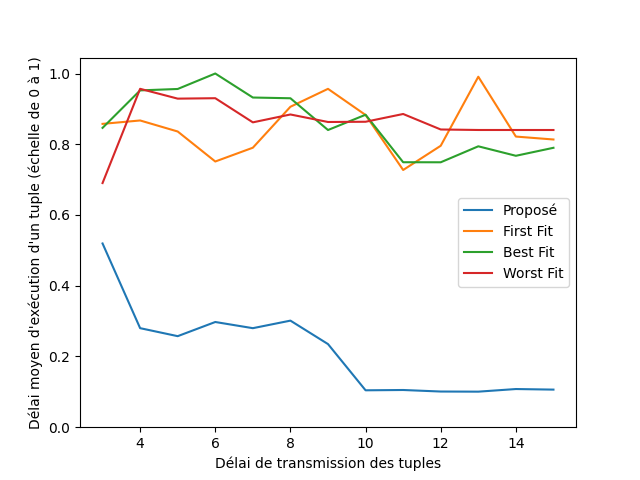
\includegraphics[]{resultats/tupleDelayT.png}
  \caption{Délai moyen d'exécution d'un tuple en fonction du taux de transmission}
  \label{fig:delai_tuple_debit}
\end{figure}

\begin{figure}[H]
  \centering
  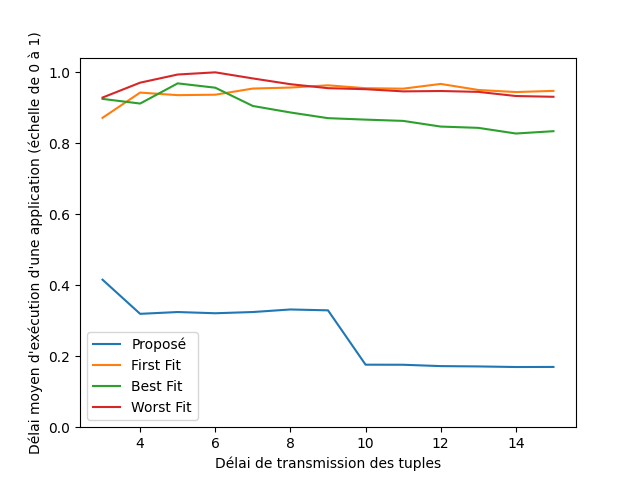
\includegraphics[]{resultats/loopDelayT.png}
  \caption{Délai moyen d'exécution d'une application en fonction du taux de transmission}
  \label{fig:delai_application_debit}
\end{figure}

Les figures \ref{fig:delai_tuple_debit} et \ref{fig:delai_application_debit} représentent, respectivement, la variation du délai d'exécution d'un tuple et le délai d'exécution d'une application selon le délai de transmission entres les tuples consécutifs.
Nous constatons que la durée d'exécution d'une application dans les stratégies classiques est stable et proche de la valeur maximale, ce qui signifie que la diminution de la charge de travail, n'influe pas sur la durée d'exécution. En revanche, la stratégie proposée démontre des performances meilleures en termes de délai ainsi qu'une réaction à la variation du délai de transmission à partir de 9 unités de temps de délai.\par

\section{Conclusion}
Nous avons réussi à montrer l'efficacité de notre technique dans la réduction du temps d'exécution des demandes de services, témoignant ainsi d'une meilleure gestion et répartition de ressources de l'ensemble des nœuds du cluster.

\chapter{Conclusion générale}
Dans ce mémoire nous avons étudié le paradigme du Fog Computing qui évolue rapidement pour atténuer les problèmes de latence, de bande passante et de qualité de service (QoS) des applications basées sur le cloud. Nous avons présenté les efforts de recherche axés sur l'optimisation de l'exploitation des ressources que propose cette architecture.\par
A notre tour, nous avons proposé un algorithme décentralisé pour la distribution équitable des demandes de services par lot sur l'ensemble de nœuds Fog organisés en clusters. Notre solution favorise la réactivité et la réduction du temps de réponse aux demandes, qui est un facteur critique pour les applications à temps réel qui expriment de grandes exigences de qualité de service. De plus, cette solution garantit la distribution équitable de charges de travail entre les nœuds d'un même cluster, ce qui permet d'éviter la saturation du réseau et la création de points critiques.\par
La solution présentée traite seulement le problème d'allocation de ressources, et peut être enrichie en explorant d'autres aspects de l'architecture Fog. Nous pouvons énumérer les perspectives suivantes permettant notamment d'éliminer les hypothèses formulées dans le chapitre de conception :
\begin{itemize}
  \item L'intégration d'un mécanisme de découverte du réseau permettant la construction d'une topologie logique de ce dernier. Ceci nous permettra de considérer le coût de la liaison réseau dans la fonction de distance entre les demandes et les nœuds proposée dans le chapitre de conception.
  \item Permettre l'ajout et le retrait dynamique de nœuds du cluster à l'aide d'une solution d'abonnement aux nœuds passerelles.
  \item Intégrer la notion de priorité entre les différentes demandes émanant des objets IoT. 
\end{itemize}
\bibliographystyle{IEEEtran}
\bibliography{references}
\newpage
\begin{tikzpicture}[remember picture,overlay]
	\draw[very thick]
	([yshift=-1cm,xshift=2cm]current page.north west)--
	([yshift=-1cm,xshift=-1cm]current page.north east)--
	([yshift=1cm,xshift=-1cm]current page.south east)--
	([yshift=1cm,xshift=2cm]current page.south west)--cycle;
\end{tikzpicture}

\thispagestyle{empty}

\begin{center}
	\Huge \color[RGB]{18,96,149} \bfseries{Conception et implémentation d'une technique d'allocation de ressources dans un environnement \emph{Fog Computing}}\\
\end{center}
\vspace{1.5 cm}
\input{ressources/résumé/ResumeFR}
\input{ressources/résumé/ResumeEN}
\end{document}